% XeLaTeX + ctex；在 docs/belf-relf/latex/ 下编译：
%   latexmk -xelatex -interaction=nonstopmode -halt-on-error belf-relf.tex

\documentclass[UTF8,a4paper,11pt]{ctexart}

\usepackage{amsmath,amssymb}
\usepackage{graphicx}
\usepackage{booktabs}
\usepackage{tabularx}
\usepackage{longtable}
\usepackage{array}
\usepackage{float}
\usepackage{hyperref}
\usepackage{geometry}
\usepackage[backend=biber,style=numeric,sorting=none]{biblatex}
\addbibresource{refs.bib}

\geometry{margin=2.5cm}
\graphicspath{{../assets/}}
\hypersetup{colorlinks=true, linkcolor=blue, citecolor=blue, urlcolor=blue}

\emergencystretch=3em

\title{bdelf BELF / RELF：设计规格与实现说明}
\author{bdelf 模型文档}
\date{\today}

\begin{document}
\maketitle

\begin{abstract}
本文档完整说明 bdelf 中两族半自回归连续语言模型 BELF 与 RELF 的动机、流几何、时间场、损失、CFG、训练接口与推理循环。
二者实现上可共享模块代码，但须分别描述、分别训练，且不共享参数。共用 ELF 约定的 rectified flow（\(t=1\) 为干净端）、token 对齐 VAE、2L pack、去噪器 \(G\)。流空间是入口输出维 \(X=\) \texttt{latent\_dim}（须与 artifact 一致）；\(D=\) \texttt{n\_embd} 只是 \(G\) 隐层。出口锁死为 \(\hat x_0\in X\) 再走 VAE-dec；主体训练损失只有 v-MSE，不含出口 CE。推理时 VAE-dec 读 token。
\textbf{BELF} 在块内未知槽共享同一标量 \(t\)，已知余数钉干净条件，块间将提交结果写入 KV cache。
\textbf{RELF} 在窗内使用降序局部时间梯子，每步自窗左端移出（pop）\(S\) 个槽；当前窗已知余数钉干净条件。
日程档 \texttt{full} 下每一族、每一档 \texttt{latent\_tune} 均须完成主训与扩展 token 预算；日程档 \texttt{mid} 仅 Stage1（\(10\mathrm{B}\) 全局批 128，\texttt{eval\_step}=1000），无扩展。生成长度上限为 \texttt{max\_seq\_len}。
工程路径见同目录上级 \texttt{README.md}。本文档不冻结 GPU 机时额度，亦不提供训练结论。
\end{abstract}

\section{动机与定位}

ELF~\cite{elf2026} 表明：在冻结上下文嵌入上，以 \(t=1\) 为干净端做线性插值，并由 x-pred 转换为速度均方误差，可在连续状态空间上完成观测恢复。其生成分解为整句共享一个标量 \(t\)、注意力全程双向，因而既无 KV cache，也不能按块提交或作可变长增量生成。Cola~\cite{cola2026} 与 AURORA-LM~\cite{aurora2026} 采用另一分解：冻结或先训练可解码 latent，再以块因果 Flow Matching 作为 prior，由独立 decoder 读出 token。该分解已是半自回归，但块内仍共享同一时间；Cola 的时间轴与 ELF 相反（\(t=0\) 为干净端），其主要主张为压缩语义 latent。

因此给出两条可分别训练与评测的半自回归 ELF：BELF 在块内未知槽共享单一时间（已知余数钉干净），RELF 在窗内使用位置相关的降序时间梯子（已知余数同样钉干净）。本文档中 VAE 将因果编码器输出映射为近似各向同性、可叠加高斯噪声的 token 对齐 latent，且不缩短序列长度。下文先陈述两族共用部分，再单开时间调度章，然后分章给出 BELF 与 RELF。本文档不设定 GPU 机时上限（5090 与 A100 均未冻结额度）。

\section{相关工作}

本节陈述近邻工作的机制及其与本规格的差异。不以 full-width latent 本身作为设计贡献。BELF 对照 AURORA、BD3-LM 与 Cola 的块因果分解；RELF 对照 Rolling Diffusion 的局部时间场，并采用 ELF 的流几何。两族分别陈述、分别训练。

\paragraph{全程一个 \(t\) 的观测恢复。}
ELF 冻结 T5 嵌入，采用 rectified flow，并由 x-pred 转换为速度均方误差。全序列双向、整句一个标量 \(t\)。CoDAR~\cite{codar2026} 将 rounding 外包给独立自回归 decoder，但仍是全序列连续扩散。二者均无已提交前缀进入 KV cache。

\paragraph{冻 AE + 块因果连续 prior。}
Cola 将 \(p(x,z_0)=p_\theta(x\mid z_0)\,p_\psi(z_0)\) 分解，并以 2L pack 一次输入干净前缀与当前块噪声。AURORA 冻结 Query-AE，对 full-width 可解码 latent 做块因果 Flow Matching。与 BELF 最近的近邻是：冻结编码器、块因果注意力、独立 decoder。BELF 当前块内已知余数采用 Cola 的 clean 条件：钉干净、只去噪未知槽。差异在于自编码器构造、流匹配配方，以及 Cola 不具备窗内降序时间梯子。

\paragraph{离散块同步 \(t\)。}
BD3-LM~\cite{bd3lm2025} 块间自回归、块内吸收态 mask、一块一个 \(t_b\)、同一网络出 logits。这是 BELF 在离散观察空间上的对应物。本规格的状态是连续 VAE 码，token 由独立出口读出。

\paragraph{视频里的局部时间滑窗。}
Rolling Diffusion~\cite{rolling2024} 将全局 \(t\) 映射为帧局部 \(t_k\)。RELF 的局部时间场在滑窗后保持时间半群一致性，其约束源于该工作。其对象为视频或物理场，而非语言模型，亦无 KV cache 与 token decoder。

\section{规格声明与设计要点}

\subsection{模型定义}

\begin{quote}
在由 \texttt{latent\_model}+\texttt{tag} 指定的 token 对齐隐空间上，以 ELF 的 rectified flow（\(t=1\) 为干净端）训练去噪器 \(G\)；推理时 \(\hat x_0\) 走 VAE-dec 读 token。\textbf{BELF} 以块内未知槽同步 \(t\) 做半自回归，当前块已知余数钉干净条件；\textbf{RELF} 以窗内降序梯子逐步 pop 做滚动半自回归，当前窗已知余数钉干净条件。该分解规定：两族均在连续隐空间上沿该流做观测恢复，并借助已提交前缀的 KV cache 生成至 \texttt{max\_seq\_len}。实现与评测以该分解为准；本文档不预设训练结论。
\end{quote}

参数分模型、训练、推理三类，见第~\ref{sec:common}~节。两族分开训练、分开评测。无并列的次要规格分支。

\subsection{设计要点}

\begin{enumerate}
  \item BELF：将同一流用于块因果 2L/KV；未知槽共享同一 \(t\)，块间默认再 encode 提交（对照 \texttt{commit\_x0hat}）；已知余数钉干净条件；\(T\) 次流均算 v-MSE；末次 Euler 后 VAE-dec 读 token（不多一次 \(G\)）。
  \item RELF：将 ELF 流几何用于滚动窗；局部时间梯子铺 \(L_0,\ldots,L_{T-1}\)，最左档 Euler 到 \(1-\varepsilon\) 后 pop。整窗 \(F\)，BOS 前 / EOS 后截断。已知余数钉干净条件。每步 pop \(S\) 个槽。训练未知真槽一律 v-MSE。
  \item 训练日程（非第三条机制贡献）：日程档 \texttt{full} 下每一族 \(\times\) 每一 \texttt{latent\_tune} 完成主训后再做扩展；日程档 \texttt{mid} 仅 Stage1（\(10\mathrm{B}@128\)，\texttt{eval\_step}=1000，\texttt{ema\_decay}=0.999）。切分见附录~\ref{sec:len}。预算与 \texttt{max\_seq\_len} 见表。日程档与 \texttt{latent\_tune=mid} 不是同一键。
\end{enumerate}

\section{共性}
\label{sec:common}

两族共用加载、映射、\(G\)、VAE-dec 读出、v-MSE 与训练日程。时间场见第~\ref{sec:time}~节。读出位置与生成循环见本族章。CFG 见第~\ref{sec:cfg}~节；提交与采样器见第~\ref{sec:infer}~节。参数表按模型 / 训练 / 推理分栏；某类无字段则省略该栏。评测长度见附录~\ref{sec:len}。

\subsection{参数三类}

超参数划分为模型、训练、推理三类。\texttt{latent\_model} 与 \texttt{tag} 属模型类：二者指定入口自编码器，因而决定入口结构，不再单列「加载」类。

\paragraph{模型。}
网络结构。必填 \texttt{latent\_model} 与 \texttt{tag}，无默认，用于调用已有加载器 \texttt{load\_latent\_artifact}。入口 encoder / decoder 在参数表里只记这两项与流维 \texttt{latent\_dim}（\(X\)，须等于 artifact 输出维）；词表、VAE 层数、s1 系数以加载结果为准，不列表。入口 encoder 的注意力块长以加载结果为准，不随本规格改写。\texttt{block\_size} 仅 BELF：\(G\) 去噪块长，100m 默认 16，主跑 \(W=T\)。加载入口块长须为 \(1\)（逐 token 因果）或等于本题 BELF \(W\)。可训档（\texttt{full} / \texttt{mid}）另要求入口块长为 \(1\)；块因果入口只允许 \texttt{frozen}。RELF 无此字段；加载入口块长必须为 \(1\)；窗长 \texttt{window\_size} 与入口无关。

\texttt{n\_embd}（记 \(D\)）是 \(G\) 的隐层宽度，与 \(X\) 无关，须整除 \texttt{n\_head}，全文只声明一次。\texttt{max\_seq\_len} 是位置编码与生成长度上限。出口锁死：无 \texttt{exit} 键、无 \texttt{linear} 对照；\(\hat x_0\in X\) 直接走加载的 VAE-dec 得 logits。主体训练不算出口 CE；VAE-dec 只在推理读出与可训档 \(\mathcal{L}_{\mathrm{s1}}\) 重建里出现。\texttt{self\_left\_prob} 进入模型指纹。

\texttt{sc\_cfg} 决定网络是否包含 ScaleEmbedder 与 self-cond 通道，因此进入模型指纹。

\paragraph{训练。}
加载之后的优化规则。\texttt{latent\_tune} 只改变梯度是否反向传播到 latent 本体，不改变加载身份。

\begin{center}
\begin{tabularx}{\textwidth}{@{}lX@{}}
\toprule
\texttt{latent\_tune} & 含义 \\
\midrule
\texttt{frozen} & 全程冻结。完整 latent 参数仍写入 s2 checkpoint。 \\
\texttt{full} & 自 step 0 起更新 latent。 \\
\texttt{mid} & 默认。已消费 token 未到 \texttt{latent\_thaw\_tokens} 时与冻结相同；到达该点后解冻一次，此后与 \texttt{full} 相同。解冻后为新可训参数分配新的优化器状态。 \\
\bottomrule
\end{tabularx}
\end{center}

\paragraph{推理。}
同一 checkpoint 上的采样规则。提交、采样器与 CFG 尺度见第~\ref{sec:infer}~节与第~\ref{sec:cfg}~节；不进入训练指纹。BELF 生成使用 \texttt{block\_generate}，RELF 生成使用 \texttt{rolling\_generate}。

第二阶段（s2）始终训练映射与 \(G\)。冻结档不计算 \(\mathcal{L}_{\mathrm{s1}}\)。
\texttt{full} 与解冻后的 \texttt{latent\_tune=mid}：只要更新 latent 的任一侧（encoder、VAE-dec、或两侧），就必须计算完整的 \(\mathcal{L}_{\mathrm{s1}}\)（重建 + \(\mathrm{KL}(q\|N(0,I))\) + BERT-mask + ref-KL）。\(\mathcal{L}_{\mathrm{s1}}\) 与 \(\mathcal{L}\) 分开相加。
主体 \(\mathcal{L}\) 只有 v-MSE，不含出口 CE。VAE-dec 参数是否更新仍只由 \texttt{latent\_tune} 决定。可训档的 \(\mathcal{L}_{\mathrm{s1}}\) 仍经同一 VAE-dec。启动时须具备 VAE-dec。\texttt{latent\_tune=mid} 解冻前仍不计算 \(\mathcal{L}_{\mathrm{s1}}\)。
速度误差仍可反向传播到 encoder；2L 左段的 \texttt{sg} 只切断 pack 左半，不切断该梯度。

\paragraph{启动校验。}
加载结果的 \(X\) 须等于配置的 \texttt{latent\_dim}；入口 encoder 块长以加载结果为准，不随 \(W\) 改写。BELF：加载入口 \texttt{encoder.block\_size} \(\in\{1,W\}\)。RELF 无 \texttt{block\_size}；加载入口块长必须为 \(1\)，且 \(S\cdot T=W\)。可训档（\texttt{latent\_tune} 的 \texttt{full} / \texttt{mid}）要求入口块长为 \(1\)，否则报错拒绝。两族 \texttt{time\_step} \(T\ge 4\)，否则报错。\(G\) 的宽度等于 \(D\)；出口锁死 VAE-dec，启动必须具备 decoder。各族额外校验见本族章。

\subsection{流、去噪器与出口}

时间：\(t=1\) 干净、\(t=0\) 纯噪。流与 v-MSE 在入口输出维 \(X=\) \texttt{latent\_dim}（须与 artifact 一致）；\(D=\) \texttt{n\_embd} 只是 \(G\) 隐层。白化留在 \(X\)，茎 \(\mathrm{Linear}(X\to D)\)，FinalLayer 回到 \(X\)：
\[
z_t=t\,x_0+(1-t)\,\varepsilon,\qquad
\hat v=\frac{\hat x_0-z_t}{\max(1-t,\,\varepsilon_t)},\qquad
v^\star=x_0-\varepsilon.
\]
\(G\) 输出干净点估计 \(\hat x_0\in\mathbb{R}^{X}\)，再转换为速度并计算 v-MSE。分母取 \(\max(1-t,\varepsilon_t)\)，其中 \(\varepsilon_t=\) \texttt{vel\_eps}，以避免 \(t\to 1\) 时除零。干净端默认取后验样本（对照均值）；推理写入 KV 的对象必须与该干净端处于同一空间 \(X\)。

\(G\) 是一份网络，不含 ELF \texttt{decoder\_prob} 双模式。条件通道为 AdaLN-Zero（DiT），不用 ELF 的 in-context control tokens（\texttt{num\_time\_tokens=0}）。块内 LayerNorm 无仿射；每层调制为 \(\mathrm{SiLU}\circ\mathrm{Linear}:D\to 6D\)，拆成 attn / MLP 的 shift、scale、gate；残差 \(x\leftarrow x+\mathrm{gate}\cdot\mathrm{sub}(\ldots)\)。调制末层权重与偏置零初始化，起步每块为恒等。FinalLayer 同样 AdaLN-Zero（调制 \(D\to 2D\) 的 shift / scale），输出线性零初始化。骨干其余不变：RoPE、qk-RMSNorm、SwiGLU。此为实现默认，不列入设计要点、不列入消融。每一层 AdaLN-Zero \textbf{逐列}以 \((t,\,w_{\mathrm{sc}},\,m)\) 为条件（\(m\) 进入模型指纹；不是序列 token，不改变 2L / 注意力）：未知列一律 \(m=\mathrm{denoise}\)，\texttt{sc\_cfg} 为真时再以 \(w_{\mathrm{sc}}\) 为条件；左段 / 已知 / PAD 不加 \(m\)、不以 \(w_{\mathrm{sc}}\) 为条件。不再设 \(m=\mathrm{decode}\)。BOS 前、EOS 后的格不在当前窗，同样不加 \(m\)。读 token 仅发生在推理时末次流 \(\hat x_0\) 之后的 VAE-dec。主体损失：未知列一律 v-MSE。左段与已知槽不进入 \(\mathcal{L}\)。BELF / RELF 均不引入 \(m_d\)/\(m_c\)。注意力与 sc 通道见本族掩码节。

主体损失只有 v-MSE（无出口 CE、无 \texttt{lambda\_ce} / \texttt{ce\_detach\_g}）：
\[
\mathcal{L}
=\lambda_{\mathrm{mse}}\,\mathcal{L}_{\mathrm{mse}}.
\]
逐 token 的 \(\|\cdot\|^2\) 对 \(X\) 取平均。BELF：抽一跳 \(i\sim\mathrm{Unif}\{0,\ldots,T-1\}\)，\(t=L_i\)，右段全部未知有效位算 v-MSE，\(m=\mathrm{denoise}\)（可 CFG）。末跳 \(t=L_{T-1}\) 不是 \(1-\varepsilon\)。已知槽不进入 \(\mathcal{L}\)。RELF 对切完后仍在窗的未知真槽平均，公式见本族掩码节。\(v_{\mathrm{tgt}}\) 是否被 CFG 修正、AdaLN 是否以 \(w_{\mathrm{sc}}\) 为条件，见第~\ref{sec:cfg}~节。可训 latent 时总目标为 \(\mathcal{L}+\mathcal{L}_{\mathrm{s1}}\)：
\[
\mathcal{L}_{\mathrm{s1}}
=\lambda_{\mathrm{vae}}\,\mathrm{CE}_{\mathrm{rec}}
+\beta\,\mathrm{KL}(q_\phi\|N(0,I))
+\lambda_{\mathrm{mask}}\,\mathcal{L}_{\mathrm{mask}}
+\lambda_{\mathrm{ref}}\,\mathrm{KL}(q_\phi\|q_{\phi_{\mathrm{ref}}}).
\]
\(\mathrm{CE}_{\mathrm{rec}}\) 与 BERT-mask 都经 VAE-dec。\(q_{\phi_{\mathrm{ref}}}\) 是 s2 开始时加载器给出的 encoder 冻结副本。\texttt{frozen} 时 \(\mathcal{L}_{\mathrm{s1}}=0\)。

网络默认分为三段：加载器编码、去噪器 \(G\)、推理时的 VAE-dec 读出。\(G\) 一律使用逐位置时间嵌入与 AdaLN-Zero；若本族各位置 \(t\) 相同，则广播同一标量。

\begin{verbatim}
tokens
  |  load_latent_artifact(latent_model, tag)
  |  Enc (block-causal) -> z in R^{S x X}
  |  optional whiten on X
  |  G stem: Linear X -> D
  v
pack_2l [sg(h_left)|h_t]
  + per-column (t, [w_sc if unknown], [m=denoise if unknown])
  -> AdaLN-Zero
  |  G: n_layer x (AdaLN-Zero -> Attn(RoPE, qk-RMSNorm)
  |                -> AdaLN-Zero -> SwiGLU)
  |  FinalLayer (AdaLN-Zero) D -> X -> x0_hat
  v
Exit (locked):  x0_hat in X -> VAE-dec  (inference readout only)
\end{verbatim}

\paragraph{出口叠法。}
出口锁死 VAE-dec：无层数键、无 \texttt{exit}、无 \texttt{linear}。\(\hat x_0\) 已在流空间 \(X\)，直接调用加载的 VAE-dec。VAE-dec 的层数 / 块长以加载结果为准，不在本规格另建。训练主体不算 CE；读出只发生在推理。

喂给 VAE-dec 的序列两族不同。推理 \texttt{block\_generate} 把已提交的干净码与当前块 \(\hat x_0\) 拼接后再取末 \(W\) 个 logits。推理 \texttt{rolling\_generate} 把 \(G\) 的整段 2L 输出送进 VAE-dec，再切右段窗。因此：BELF 推理前缀是提交码而不是 \(G\) 左段输出；RELF 读出前缀是 \(G\) 左段的 \(\hat x_0\)。

2L 与 Cola 块因果结构同构：已完成段写入 KV 后组内双向、组间单向；右段可见左段。BELF 的组是本规格 \texttt{block\_size} \(W\)；RELF 已完成段按加载入口块长（必须为 1，即逐 token 因果），窗内组是档 \(S\)。左段 \(t=1\)，不加 \(m\)，AdaLN-Zero 不以 \(w_{\mathrm{sc}}\) 为条件。\texttt{sc\_cfg} 为真时右段未知槽（一律 \(m=\mathrm{denoise}\)）再以 \(w_{\mathrm{sc}}\) 为条件。推理时末次流的 \(\hat x_0\) 走 VAE-dec；\(\mathcal{L}_{\mathrm{s1}}\) 仍只用它做重建。\(G\) 的注意力可见性按本族掩码节落地。时间梯子与各族如何铺 \(t\)，见第~\ref{sec:time}~节。

\paragraph{self-left。}
\label{sec:self-left}
推理左段默认是再 encode 采 \(z\) 写入的码（对照 \texttt{commit\_x0hat} 才提交 \(\hat x_0\)）；训练默认仍是 encoder 干净码。以概率 \texttt{self\_left\_prob}（默认 \(0.25\)，eval / 生成视为 0）按样本把左段换成 stop-grad 的末流 \(\hat x_0\)：在 CFG 之前，用 GT 左 + 右段钉 \(t=L_{T-1}\)、\(m=\mathrm{denoise}\) 做一次 \texttt{no\_grad} \(G\)（与推理末跳同条件，取 x-pred，不 Euler），Bernoulli 替换 \(h_{\mathrm{left}}\)，再跑 teacher / 学生。已知余数与 PAD 仍钉 encoder 干净码。这不是当前训练 hop 的 \(\hat x_0\)。BELF 与 RELF 共用。

\subsection{日程与 checkpoint}

Token 预算：日程档 \texttt{full} 下每族 \(\times\) 每一 \texttt{latent\_tune} 各有主训与扩展两份，不共用（\(B_{\mathrm{main}}\) / \(B_{\mathrm{ext}}\) 见表）。日程档 \texttt{mid} 仅 Stage1（\(B_{\mathrm{mid}}=10\mathrm{B}\)，全局序列批 128，\texttt{eval\_step}=1000，\texttt{ema\_decay}=0.999），无扩展。切分长度与档比见附录~\ref{sec:len}。工程上主训与扩展是两次独立训练（不同 preprocess / 不同 checkpoint 哈希），扩展可用更大显存的卡。扩展启动时要求同参主训已正常结束，并从主训 \texttt{checkpoint\_latest} 的 EMA 初始化 live 权重（不恢复优化器）。\texttt{latent\_tune=mid} 的解冻点落在主训内；若主训已过解冻点，扩展立即保持解冻。checkpoint 变体为 \texttt{fast} / \texttt{mid} / \texttt{full}（路径 \texttt{cache/checkpoints/\{fast|mid|full\}/\ldots}），与 \texttt{latent\_tune=mid} 不是同一键。

新 run 自 step 0 调用 \texttt{load\_latent\_artifact}，扩展 run 再被主训 EMA 覆盖。此后只使用本 run 的 checkpoint 中的 latent 副本。无论是否训练 latent，该 checkpoint 都必须包含完整 latent 参数。同一 Stage 续训先读取本 run，再按累计 token 判断是否已超过 \texttt{latent\_thaw\_tokens}。
模型类字段进入模型指纹（包括 \texttt{latent\_model}+\texttt{tag}、\texttt{sc\_cfg}、\texttt{self\_left\_prob}）；训练类进入训练指纹（包括 \texttt{latent\_tune}）。现网只有一份训练哈希 \texttt{build\_train\_fingerprint}：整份 model YAML（含 \texttt{sampling}）与 \texttt{generate\_cfg} 一并纳入；推理字段因此也会换 run 目录。规格分类上的「推理不进训练指纹」与此现网行为分开：本次不改全局管线。

\subsection{共性参数}

下表为 100m 规模默认值。修改默认值须写入对应指纹。\(G\) 与优化器内部见附录。入口 encoder / decoder 只记 \texttt{latent\_model} 与 \texttt{tag}。

{\small
\begin{center}
\begin{tabularx}{\textwidth}{@{}l c X l@{}}
\toprule
名称 & 符号 & 释义 & 默认 \\
\midrule
\multicolumn{4}{@{}l}{\textit{模型（共用）}} \\
\texttt{latent\_model} & & 交给 \texttt{load\_latent\_artifact} 的家族名。 & 必填 \\
\texttt{tag} & & 交给加载器的 tag。 & 必填 \\
\texttt{n\_embd} & \(D\) & \(G\) 隐层宽。与流空间 \(X\) 无关。 & \(768\) \\
\texttt{latent\_dim} & \(X\) & 流空间维；须等于 artifact 输出维。 & \(32\) \\
\texttt{max\_seq\_len} & & 位置编码与生成长度上限。 & \(4096\) \\
\texttt{self\_left\_prob} & \(p_{\mathrm{left}}\) & 训练时按样本把 2L 左段换成末流 \(\mathrm{sg}(\hat x_0)\) 的概率；eval / 生成视为 0。 & \(0.25\) \\
\midrule
\multicolumn{4}{@{}l}{\textit{训练（共用）}} \\
\texttt{latent\_tune} & & 加载之后是否训练 latent 本体。三档对应三个训练配置哈希。与日程档 \texttt{mid} 不是同一键。 & \texttt{mid} \\
\texttt{latent\_thaw\_tokens} & & 仅 \texttt{latent\_tune=mid} 的解冻点。 & \(15\mathrm{B}\) \\
\texttt{target\_tokens} & \(B_{\mathrm{main}}\) & 日程档 \texttt{full} 的主训预算（每族 \(\times\) 每一 \texttt{latent\_tune}）。 & \(45\mathrm{B}\) \\
\texttt{ext\_tokens} & \(B_{\mathrm{ext}}\) & 日程档 \texttt{full} 的扩展预算。日程档 \texttt{mid} 无此项。 & \(5\mathrm{B}\) \\
\texttt{mid\_tokens} & \(B_{\mathrm{mid}}\) & 日程档 \texttt{mid} 仅 Stage1 的预算。 & \(10\mathrm{B}\) \\
\bottomrule
\end{tabularx}
\end{center}
}

全局推理参数见第~\ref{sec:infer}~节。CFG 见第~\ref{sec:cfg}~节。时间调度参数见第~\ref{sec:time}~节。

\paragraph{消融。}
对照按下列网格执行。\texttt{latent\_tune} 三档为主网格：日程档 \texttt{full} 下每族 \(\times\) 每一档各走主训与扩展预算（见表），不计入短训消融。其余训练短训不占用主跑 token 预算，建议每条使用扩展预算（切分见附录~\ref{sec:len}）。无出口 CE，故无 \texttt{ce\_detach\_g}。各表按模型 / 训练 / 推理分栏。全局推理消融见第~\ref{sec:infer}~节。

{\small
\setlength{\tabcolsep}{4pt}
\begin{center}
\begin{tabularx}{\textwidth}{@{}
  >{\raggedright\arraybackslash}p{0.22\textwidth}
  c
  >{\raggedright\arraybackslash}p{0.16\textwidth}
  >{\raggedright\arraybackslash}X
  @{}}
\toprule
名称 & 符号 & 默认 & 对照 \\
\midrule
\multicolumn{4}{@{}l}{\textit{模型}} \\
\texttt{self\_left\_prob} & \(p_{\mathrm{left}}\) & \(0.25\) & \(\{0,0.125,0.25,0.375,0.5\}\) \\
\midrule
\multicolumn{4}{@{}l}{\textit{训练}} \\
\texttt{latent\_tune} & & \texttt{mid} & \texttt{frozen}、\texttt{full}（主网格；日程档 \texttt{full} 下每档各走 \(B_{\mathrm{main}}+B_{\mathrm{ext}}\)） \\
\texttt{x0\_source} & & \texttt{z} & \texttt{mu} \\
\bottomrule
\end{tabularx}
\end{center}
}


\section{时间调度}
\label{sec:time}

两族共用同一把确定梯子 \(\{L_i\}\)。档数 \(T\)（\texttt{time\_step}）由本族给出。不另设调度器开关。共性给出 \(Q\) 与 \(\{L_i\}\)；BELF / RELF 两小节给出如何把梯子铺到块或窗。

\subsection{共性}

设 \(Z\sim\mathcal{N}(0,1)\)。\(\Phi\) 是它的累积分布函数
\[
\Phi(z)=P(Z\le z)=\int_{-\infty}^{z}\frac{1}{\sqrt{2\pi}}\,e^{-u^{2}/2}\,du,
\]
\(\Phi^{-1}\) 是分位函数：对 \(p\in(0,1)\) 有 \(\Phi\bigl(\Phi^{-1}(p)\bigr)=p\)。实现为 \(\Phi^{-1}(p)=\sqrt{2}\,\mathrm{erfinv}(2p-1)\)。\(p\to 0^{+}\) 时 \(\Phi^{-1}(p)\to-\infty\)，\(p\to 1^{-}\) 时 \(\to+\infty\)，故端点必须特判。

训练时间取 \(t=\sigma(P_m+P_s Z)\)，即 \(\mathrm{logit}(t)\sim\mathcal{N}(P_m,P_s^{2})\)，其中 \(\sigma(u)=(1+e^{-u})^{-1}\)。该分布的分位函数为
\[
Q(p)=\begin{cases}
0 & p=0,\\
\sigma\bigl(P_m+P_s\,\Phi^{-1}(p)\bigr) & 0<p<1,\\
1-\varepsilon & p=1.
\end{cases}
\]
开区间结果再夹到 \([0,1-\varepsilon]\)。\(P_m,P_s,\varepsilon\) 见本节参数表。

档位在\textbf{概率轴}上等分，不是在 \(t\) 上等间隔。\texttt{time\_step} \(T\) 是每块 / 每窗的\textbf{流}步数（亦为 \(G\) 次数；RELF 仍 \(S\cdot T=W\)）。须 \(T\ge 4\)，否则启动报错拒绝。主体无出口 CE，不再另留 decode 跳；概率轴按 \(T\) 均分（\(T+1\) 个点）：
\[
L_i=Q\!\left(\frac{i}{T}\right),\qquad i=0,1,\ldots,T.
\]
因而 \(L_0=0\)，\(L_T=Q(1)=1-\varepsilon\)。第 \(i\) 跳（\(i=0,\ldots,T-1\)）在 \(t=L_i\) 上跑 \(G\)，\(\Delta t=L_{i+1}-L_i\)，末次 Euler 到 \(1-\varepsilon\)。推理用末次流的 \(\hat x_0\) 走 VAE-dec，不再于 \(t=1-\varepsilon\) 多跑一次 \(G\)。默认 \(T=16\)、\(P_m=0\)、\(P_s=0.8\)。训练与推理共用该确定梯子：推理不再从 logit-normal 随机采样，也不使用 \(\mathrm{linspace}(0,1)\)。

{\small
\begin{center}
\begin{tabularx}{\textwidth}{@{}l c X l@{}}
\toprule
名称 & 符号 & 释义 & 默认 \\
\midrule
\multicolumn{4}{@{}l}{\textit{模型（共用）}} \\
\texttt{denoiser\_p\_mean} & \(P_m\) & \(\mathrm{logit}(t)\sim\mathcal{N}(P_m,P_s^{2})\) 的均值。 & \(0\) \\
\texttt{denoiser\_p\_std} & \(P_s\) & 同上，标准差。 & \(0.8\) \\
\texttt{t\_clean\_eps} & \(\varepsilon\) & \(Q(1)=L_T=1-\varepsilon\)；末次 Euler 终点。窗 / 训练 hop 不到此点。 & \(0.05\) \\
\bottomrule
\end{tabularx}
\end{center}
}

\subsection{BELF}
\label{sec:belf-t}

\texttt{train\_t\_schedule=block}。梯子按上一小节：\(L_i=Q(i/T)\)，\(i=0,\ldots,T\)。每次前向采样一跳 \(i\sim\mathrm{Unif}\{0,\ldots,T-1\}\)，将该跳 \(t=L_i\) \textbf{广播到当前块的未知槽}。
全部跳未知槽 \(m=\mathrm{denoise}\)，监督该跳流的信噪比（v-MSE；\(g=1\) 时可按 CFG 修正 \(v_{\mathrm{tgt}}\)），以 \(w_{\mathrm{sc}}\) 为条件。末跳 \(t=L_{T-1}\)，不是 \(1-\varepsilon\)。
已知槽钉 \(t=1\)，不加 \(m\)、不加噪。主跑 \(W=T\)。切块对齐 \(0,W,2W,\ldots\)。已提交的完整块进入 KV，流仅作用于当前块的未知槽。推理 \texttt{block\_generate} 共 \(T\) 次 \(G\)：跳 \(i=0,\ldots,T-1\) 未知槽 \(t=L_i\)，Euler \(\Delta t=L_{i+1}-L_i\)（末流从 \(L_{T-1}\) 走到 \(1-\varepsilon\)）；然后用末次 \(\hat x_0\) 走 VAE-dec，不多一次 \(G\)。已知槽每跳钉 \(t=1\) 并覆写为 encoder 干净码。混合块如何自生成、如何训，见第~\ref{sec:belf-clean}~节。

\subsection{RELF}
\label{sec:relf-t}

\texttt{train\_t\_schedule=mixed}。不设 \texttt{p\_preroll} / \texttt{p\_freeroll} / \texttt{p\_postroll}，也不按 Cat 抽支。梯子按共性小节：\(L_i=Q(i/T)\)，\(i=0,\ldots,T\)。时间场以\textbf{档}为单元：每档 \(S\) 槽共享同一流起点（窗内铺 \(L_0,\ldots,L_{T-1}\)；\(L_T=1-\varepsilon\) 只作 Euler 终点）。未知档每步只升\textbf{一档}（接到更高的 \(L_i\)，最左档从 \(L_{T-1}\) Euler 到 \(1-\varepsilon\)）。每次前向只指定当前窗的一帧 \(t\) 场。

先构造\textbf{整窗} freeroll 场 \(F\)：位置 \(k=0,\ldots,W-1\)，
\[
F_k = L_{T-1-\lfloor k/S\rfloor}.
\]
即档 \(r=0,\ldots,T-1\) 占槽 \([rS,(r+1)S)\)，值为 \(L_{T-1-r}\)。最左档 \(t=L_{T-1}\)（末流起点），右组纯噪 \(L_0\)。窗内不铺 \(L_T=1-\varepsilon\)。这把 \(F\) 是唯一模板。

截断看 \textbf{BOS / EOS 落在虚拟满窗的哪一格}，不是先抽档数再把 \(F\) 左右搬去凑满 \(W\)。记 BOS、EOS 的文档下标为 \(i_{\mathrm{bos}}\)、\(i_{\mathrm{eos}}\)（均含该 token）。PAD 不是边界。窗起点 \(u\) 按文档起点 \(S\) 格对齐，覆盖 \([u,u+W)\)。对窗内格 \(k=0,\ldots,W-1\)，文档下标 \(j=u+k\)：
\begin{itemize}
  \item \(j<i_{\mathrm{bos}}\)：\textbf{BOS 之前}，整段丢掉，不在当前窗。
  \item \(j>i_{\mathrm{eos}}\)：\textbf{EOS 之后}，整段丢掉，不在当前窗。
  \item 否则：真槽，\(t_k=F_k\)（沿用满窗 \(F\) 在该格上的值）。
\end{itemize}
丢掉的位置不赋 \(t=0\)、不赋末流终点 \(1-\varepsilon\)，也不把留下的梯子挪到另一头去凑满 \(W\)。真窗可以短于 \(W\)。

两种切法相互独立、可以叠加，不是互斥分区。对虚拟满窗 \(F\)：
\begin{itemize}
  \item \textbf{句首切（preroll）}：\(j<i_{\mathrm{bos}}\) 的格丢掉。BOS 落在窗内格 \(k_{\mathrm{bos}}=i_{\mathrm{bos}}-u\)，\textbf{其左全部截掉}。
  \item \textbf{句尾切（postroll）}：\(j>i_{\mathrm{eos}}\) 的格丢掉。EOS 落在窗内格 \(k_{\mathrm{eos}}=i_{\mathrm{eos}}-u\)，\textbf{其右全部截掉}。
\end{itemize}
两端都不切（\(u\ge i_{\mathrm{bos}}\) 且 \(u+W-1\le i_{\mathrm{eos}}\)）则整窗 \(t\leftarrow F\)（句中 / freeroll）。只切左留下 \(F\) 的右侧（更噪）；只切右留下 \(F\) 的左侧（更净）；都切留下 \(F\) 的中段。损失按切完后的格计算，见第~\ref{sec:relf-mask}~节。

抽窗须使交集非空。做了句首切则真窗含 BOS；做了句尾切则真窗含 EOS。禁止为凑档把 BOS / EOS 挪出真槽；禁止把 PAD 当截断对象。BOS / EOS 不必落在档界上；所在档被截成短档时，留下的槽仍用该档的 \(F_k\)。

禁止：将 token 窗对齐铺满为从 BOS 起的 \(W\)、把最噪档搬到窗左、右侧铺 \(t=0\)「尚未进入」；禁止把 \(F\) 左侧截掉再把剩余滑到窗右。

窗内时间场锁死为梯子（\texttt{window\_t=ladder}），不进消融。不对齐前缀的余数走左切爬梯（与 preroll 同构），不是钉在满窗 \(F\) 左侧一次读出；句首切不抽 \(r\)。见第~\ref{sec:relf-clean}~节。

\section{CFG}
\label{sec:cfg}

CFG 含两根相互独立的轴。\(w_{\mathrm{sc}}\) 进入右段未知槽 AdaLN（未知一律 \(m=\mathrm{denoise}\)）。推理为单次前向。\(w_{\mathrm{ctx}}\) 在训练时以概率丢弃前缀；推理默认仅运行带前缀的一次前向，外推时另需无前缀支路，共两次前向。推理时 VAE-dec 只读取末次流的 \(\hat x_0\)。无「纯 decode 步」：每跳都可跑 teacher。

\subsection{\texorpdfstring{\(w_{\mathrm{sc}}\)：self-cond CFG}{w_sc：self-cond CFG}}

条件对象为上一跳的 \(\hat x_0\)。启用时 \(w_{\mathrm{sc}}\) 进入 AdaLN 的 \texttt{ScaleEmbedder}，与 \(t\) 的 \texttt{TimestepEmbedder} 分开。推理为单次前向。

\paragraph{启动开关。}
\texttt{sc\_cfg} 默认 \texttt{true}，进入模型指纹，因其决定网络是否包含 ScaleEmbedder 与 self-cond 通道。为真时必须具备 sc 通道。训练启动时若设为 \texttt{false}：不构建 ScaleEmbedder、无 sc 通道、AdaLN 不以 \(w_{\mathrm{sc}}\) 为条件（仍逐列加 \(m\)）、\(v_{\mathrm{tgt}}=v_z\)、不做 teacher 的 \(\Delta v\) 前向；推理忽略 \texttt{w\_sc}。\texttt{sc\_cfg} 为真则 \texttt{self\_cond=true}。

\paragraph{训练采样。}
\texttt{sc\_cfg} 为真时，每个样本独立采样两项：
\begin{enumerate}
  \item \(w_{\mathrm{sc}}\)：对齐 ELF，在 logit-normal 上采样后再仿射到给定区间，而非在该区间上均匀采样。先采样
  \[
  z\sim\mathcal{N}(P_m^{\mathrm{sc}},(P_s^{\mathrm{sc}})^2),\quad
  u=\sigma(z),
  \]
  再按 ELF \texttt{sample\_cfg\_scale} 映到区间：
  \[
  a=1+w^{\mathrm{sc}}_{\min},\quad b=1+w^{\mathrm{sc}}_{\max},\quad
  w_{\mathrm{sc}}=a\,(b/a)^{u}-1.
  \]
  \(P_m^{\mathrm{sc}},P_s^{\mathrm{sc}}\) 见表；\(w^{\mathrm{sc}}_{\min},w^{\mathrm{sc}}_{\max}\) 见附录。该分布既不是 \(\mathrm{Unif}[w^{\mathrm{sc}}_{\min},w^{\mathrm{sc}}_{\max}]\)，也不是对 \(w_{\mathrm{sc}}\) 本身的 \(\mathrm{LogUnif}\)。
  \item \(g\sim\mathrm{Bern}(\texttt{sc\_guided\_prob})\)：是否按 CFG 修正速度目标，以及是否将 uncond 的 \(\hat x_0\) 写入 sc 通道。
\end{enumerate}
\(g=0\) 时仍采样 \(w_{\mathrm{sc}}\) 并写入右段未知槽 AdaLN，使推理所用的 \(w_{\mathrm{sc}}\) 落在训练边缘分布内。\texttt{sc\_cfg} 为假时不采样这两项。

\paragraph{启用时的一次 step。}
三次前向使用同一个已采样的 \(w_{\mathrm{sc}}\)（两个 teacher \texttt{no\_grad}，一个学生），\(w_{\mathrm{sc}}\) \textbf{写入右段未知槽} AdaLN：

\begin{enumerate}
  \item Teacher uncond：self-cond 通道全 \(0\) \(\to\hat x_0^{u},\,v_u\)。
  \item Teacher cond：通道 \(\mathrm{sg}(\hat x_0^{u})\) \(\to v_c\)。
  \item 学生：未知列对 \(v_{\mathrm{tgt}}\) 计算 v-MSE。
\end{enumerate}

\[
v_{\mathrm{tgt}}=\begin{cases}
v_z+\bigl(1-1/w_{\mathrm{sc}}\bigr)(v_c-v_u) & g=1,\\
v_z & g=0.
\end{cases}
\]
CFG 对 \(v_{\mathrm{tgt}}\) 的修正施加于右段未知列。
\(g=1\) 时学生的 sc 通道为 \(\mathrm{sg}(\hat x_0^{u})\)；\(g=0\) 时通道为 \(0\)（未知槽 AdaLN 仍以已采样的 \(w_{\mathrm{sc}}\) 为条件）。左段与已知槽 AdaLN 不以 \(w_{\mathrm{sc}}\) 为条件。提交与 \texttt{forward\_clean} 同左段。Teacher 的 \(\Delta v\) 对目标 stop-grad。

BELF：未知槽共享同一套 sc。已知槽 sc 为 0。RELF：即使 \(g=1\)，窗内最右 \(S\) 个新噪声槽的 sc 仍为 \(0\)（尚无上一跳估计）。左段与干净槽的 sc 为 \(0\)。最左档与其余未知档同样以 \(w_{\mathrm{sc}}\) 为条件。

推理：未知槽 sc 为上一步提交的 \(\hat x_0\)（序列开始或新块/新槽/已知槽为 \(0\)）；未知槽 AdaLN 以推理 \(w_{\mathrm{sc}}\) 为条件。前缀 KV 不随 \(w_{\mathrm{sc}}\) 重算。

\subsection{\texorpdfstring{\(w_{\mathrm{ctx}}\)：上下文 CFG}{w_ctx：上下文 CFG}}

条件对象为 2L 左段 / KV 前缀，与 \(w_{\mathrm{sc}}\) 独立，不进入 AdaLN。

\paragraph{训练采样。}
每个样本再独立采样 \(d\sim\mathrm{Bern}(p_{\mathrm{drop}}^{\mathrm{ctx}})\)（与 \(g\)、\(w_{\mathrm{sc}}\) 均独立）。\(d=1\) 时丢弃 2L 左段，仅训练当前块/窗。此为训练期的无条件上下文。

推理默认仅运行带前缀的一次前向。若对 \(w_{\mathrm{ctx}}\) 做外推：无条件支路为\textbf{无前缀、仅运行当前块/窗}。然后
\[
v=v_{\mathrm{u}}^{\mathrm{ctx}}+w_{\mathrm{ctx}}\bigl(v_{\mathrm{c}}^{\mathrm{ctx}}-v_{\mathrm{u}}^{\mathrm{ctx}}\bigr).
\]
消融取值见表。

\subsection{CFG 参数}

{\small
\begin{center}
\begin{tabularx}{\textwidth}{@{}l c X l@{}}
\toprule
名称 & 符号 & 释义 & 默认 \\
\midrule
\multicolumn{4}{@{}l}{\textit{模型}} \\
\texttt{sc\_cfg} & & 是否启用整套 \(w_{\mathrm{sc}}\)（含 sc 通道）。为假则无通道、不构建 ScaleEmbedder、不以 CFG 修正 \(v_{\mathrm{tgt}}\)。进入模型指纹。 & \texttt{true} \\
\midrule
\multicolumn{4}{@{}l}{\textit{训练}} \\
\texttt{self\_cond\_cfg\_p\_mean} & \(P_m^{\mathrm{sc}}\) & 训练 \(w_{\mathrm{sc}}\) 的 logit-normal 位置。对齐 ELF 原时间场，不随梯子 \(P_m\) 改。 & \(-1.5\) \\
\texttt{self\_cond\_cfg\_p\_std} & \(P_s^{\mathrm{sc}}\) & 尺度。 & \(0.8\) \\
\texttt{sc\_guided\_prob} & \(p_g^{\mathrm{sc}}\) & 仅 \texttt{sc\_cfg}：本 step 按 CFG 修正速度目标并写入 sc 通道的概率。 & \(0.5\) \\
\texttt{ctx\_p\_drop} & \(p_{\mathrm{drop}}^{\mathrm{ctx}}\) & 丢弃 2L 左段的概率。与 \(g\) 独立。不进消融。 & \(0.1\) \\
\midrule
\multicolumn{4}{@{}l}{\textit{推理}} \\
\texttt{w\_sc} & \(w_{\mathrm{sc}}\) & 推理尺度。\texttt{sc\_cfg=false} 的 ckpt 忽略。YAML / \texttt{sampling} 键名即此；实现仍接受 ELF 别名 \texttt{self\_cond\_cfg\_scale}，但已写 \texttt{w\_sc} 时别名不生效。 & \(2.0\) \\
\texttt{w\_ctx} & \(w_{\mathrm{ctx}}\) & 推理上下文外推；\(1\)=不外推。YAML 键名即此；别名 \texttt{ctx\_cfg\_scale} 同上。 & \(1.0\) \\
\bottomrule
\end{tabularx}
\end{center}
}

训练 \(w_{\mathrm{sc}}\) 的 logit-normal 参数见表；采样区间 \(w^{\mathrm{sc}}_{\min},w^{\mathrm{sc}}_{\max}\) 见附录。推理 \(w_{\mathrm{ctx}}\) 允许区间 \(w^{\mathrm{ctx}}_{\min},w^{\mathrm{ctx}}_{\max}\) 见附录。推理尺度可在同一 checkpoint 上更改，不进入训练指纹。仅 \texttt{sc\_cfg=true} 训练得到的 run 才对推理 \(w_{\mathrm{sc}}\) 做扫描；前缀 KV 不随 \(w_{\mathrm{sc}}\) 重算。\texttt{sc\_cfg=false} 的 run 不对 \(w_{\mathrm{sc}}\) 扫描。全局提交、采样器与温度见第~\ref{sec:infer}~节。

\subsection{CFG 消融}

对照按下列网格执行。\texttt{sc\_cfg} 须单独短训；推理项使用同一 checkpoint。按槽拆损失已确定，见第~\ref{sec:open}~节，不作为消融项。\texttt{ctx\_p\_drop} 不进消融。

{\small
\setlength{\tabcolsep}{4pt}
\begin{center}
\begin{tabularx}{\textwidth}{@{}
  >{\raggedright\arraybackslash}p{0.22\textwidth}
  c
  >{\raggedright\arraybackslash}p{0.16\textwidth}
  >{\raggedright\arraybackslash}X
  @{}}
\toprule
名称 & 符号 & 默认 & 对照 \\
\midrule
\multicolumn{4}{@{}l}{\textit{模型}} \\
\texttt{sc\_cfg} & & \texttt{true} & \texttt{false}（训练启动时关闭整套 \(w_{\mathrm{sc}}\)，无 sc 通道） \\
\midrule
\multicolumn{4}{@{}l}{\textit{推理}} \\
\texttt{w\_sc} & \(w_{\mathrm{sc}}\) & \(2\) & \(\{0.5,1,2,3\}\)；仅 \texttt{sc\_cfg=true} \\
\texttt{w\_ctx} & \(w_{\mathrm{ctx}}\) & \(1\) & \(\{1,2,3,5,7\}\) \\
\bottomrule
\end{tabularx}
\end{center}
}

\section{BELF}
\label{sec:belf}

块半自回归。联合分布写成 \(p(z_0)=\prod_b p_G(z_0^{(b)}\mid z_0^{(<b)})\)。每一块是一条条件 rectified flow：\textbf{未知槽共享同一标量 \(t\)}；已知余数钉 \(t=1\)。去噪块长等于本规格 \texttt{block\_size}（\(W\)）：100m 默认 16，主跑 \(W=T\)。加载入口块长须 \(\in\{1,W\}\)；可训档另要求入口块长为 \(1\)。入口 encoder 仍按其加载块长做块因果，不随 \(W\) 改写。训练均匀采样跳号 \(i\sim\mathrm{Unif}\{0,\ldots,T-1\}\)，对该跳全部未知有效位算 v-MSE。对照 \(W=1\) 时 \(T\) 仍见表，不强制 \(T=1\)。若将 \(W\) 与 \(T\) 分开设置，须写入指纹。当前块内已知余数如何自生成、如何训，见第~\ref{sec:belf-clean}~节。

\subsection{Clean}
\label{sec:belf-clean}

主跑 \texttt{cond\_mode=clean}。本节规定两件事：\textbf{自生成}（推理时已知余数与已提交前缀从哪来）和 \textbf{训练}（如何抽到同构的混合块）。损失与注意力见第~\ref{sec:belf-mask}~节。

\paragraph{格子。}
切块对齐 \(0,W,2W,\ldots\)。前缀长 \(L\) 时 \(r=L\bmod W\)。完整块 \(\lfloor L/W\rfloor\) 进入 KV；当前块起点 \(\lfloor L/W\rfloor\cdot W\)。末块可短只指序列末端不够一整块。\(r=0\) 时当前块没有已知余数。\(W=1\) 时 \(r\) 恒为 0，clean 不触发、不抽混合块。

\paragraph{自生成。}
\texttt{block\_generate} 给定前缀 token（长 \(L\)）：
\begin{enumerate}
  \item \textbf{已齐的完整块}写入 KV。同一次生成循环里刚写完的块默认 \texttt{commit\_x0hat=false}：先 VAE-dec 读出再 encode \textbf{采 \(z\)} 写入。对照 \texttt{true} 才把 \(G\) 的 \(\hat x_0\) 提交、不再 encode。若这次调用的前缀是外部文本（提示，或上一轮已经写出再当作新前缀），完整块走 encoder 再按第~\ref{sec:infer}~节提交。这是左段干净条件，不是当前块内的余数。
  \item \textbf{当前块已知余数}只在 \(r>0\) 时出现：槽 \([0,r)\) 钉 \(t=1\)，码是前缀对应位置的 encoder 干净码，不进入损失。这 \(r\) 个 token 可以是提示，也可以是上一轮已写出、这次当新前缀的自生成 token。\(r=0\) 则整块未知。
  \item 未知槽从噪声走 \(T\) 次流。每跳之后把已知槽覆写回 encoder 干净码并钉 \(t=1\)，避免 Euler / SDE 冲掉已知位。末次 Euler 后用该跳 \(\hat x_0\) 读出。
  \item 出口读整块 token，丢掉已知槽对应位置，只保留新写的。再把本块按第~\ref{sec:infer}~节提交进 KV。此后下一块整块未知：自生成的完整块只出现在左段 KV，不再以块内余数出现。
  \item 一块一次读出。不会在同一块内把刚 decode 的 token 立刻改成已知余数再继续流。EOS 停。
\end{enumerate}

\paragraph{训练。}
以概率 \texttt{clean\_block\_prob} 把当前块抽成混合块：有效长 \(W'\)（末块可短），切点 \(r\sim\mathrm{Unif}\{1,\ldots,W'-1\}\)。槽 \([0,r)\) 为已知（\(t=1\)、不进损失），\([r,W')\) 为未知（走该跳 \(t=L_i\)）。其余前向整块均为未知。\(W=1\) 或 \(W'\le 1\) 时不抽混合块。已知槽始终是 encoder 码，不用 \(\hat x_0\) 冒充余数。右段 unknown Q 不可见同块 PAD K。可训档硬拒入口块长 \(\neq 1\)，不必二次 encode。仅冻结档且入口块长 \(=W\) 时，余数再 encode 一份条件句（当前块 \([r,W)\) 写成 PAD），已知覆写与 PAD 干净码用这份；插值靶仍来自整句 encode。左段 KV 训练时默认是 encoder 干净码（教师强制），以概率 \texttt{self\_left\_prob} 换成末流 \(\mathrm{sg}(\hat x_0)\)（见第~\ref{sec:self-left}~节）；推理左段默认是再 encode 采 \(z\)。

\paragraph{排除项。}
不随机挪块界。任意位置填空（左右都有干净上下文）须改 2L 可见性，不在本文档范围。

\begin{figure}[H]
\centering
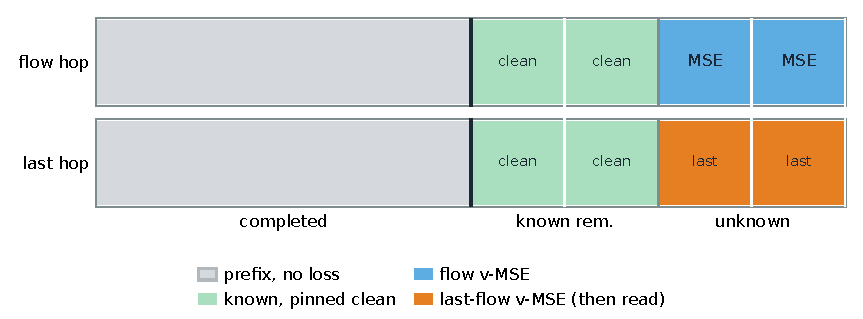
\includegraphics[width=0.72\textwidth]{belf_clean.pdf}
\caption{BELF clean：当前块左侧为已知余数，钉干净、不进损失；右侧未知槽走块内同一 \(t\)。橙为末流档（仍是 v-MSE）。}
\label{fig:belf-clean}
\end{figure}

续写见图~\ref{fig:belf-clean-cont}：前缀对不齐块界时，先在当前块未知槽上走完 \(T\) 次流、只读出新词并提交整块；此后下一块整块未知。

\begin{figure}[H]
\centering
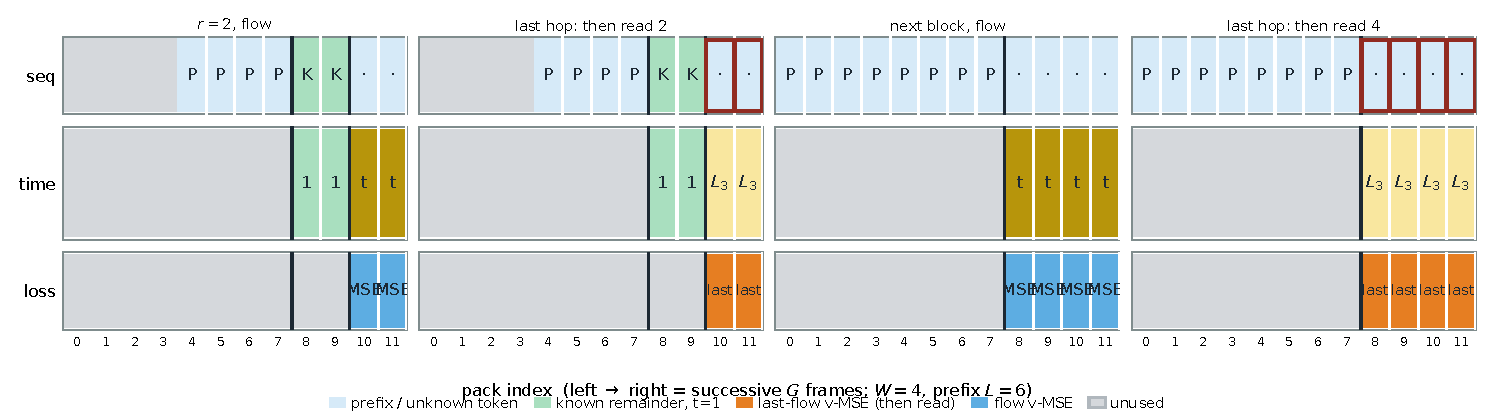
\includegraphics[width=\textwidth]{belf_clean_cont.pdf}
\caption{BELF clean 续写（\(W=4\)，前缀 \(L=6\) 故 \(r=2\)）。从左到右为相继的 \(G\) 帧。在混合块未知槽上走完流后读出 2 个新词；提交后下一块整块未知。绿格为块内已知余数（\(t=1\)，不进损失）。流跳只画一帧（未知槽同一 \(t\)）。红框为该帧读出的新词。}
\label{fig:belf-clean-cont}
\end{figure}

\subsection{训练}

加载并按 \texttt{latent\_tune} 编码，按 \(W\) 切块（主训切分见附录~\ref{sec:len}），映射后 2L pack。CFG 采样见第~\ref{sec:cfg}~节。切块对齐 \(0,W,2W,\ldots\)。\textbf{训练要求}序列长度被 \(W\) 整除，否则报错拒绝；混合块余数按满块 \(W\) 抽取 \(r\sim\mathrm{Unif}\{1,\ldots,W-1\}\)，不按短末块有效长 \(W'\)。推理末块可短，见第~\ref{sec:belf}~节推理。是否混合块、已知槽如何钉干净，见第~\ref{sec:belf-clean}~节。按第~\ref{sec:belf-t}~节指定右段时间并加噪：未知槽 \(t=L_i\)；已知槽见 Clean 节。

未知槽 \(z_t=t x_0+(1-t)\varepsilon\)。右段全部未知有效位计算 v-MSE：各跳 \(m=\mathrm{denoise}\)（可 CFG），\(t=L_i\)。已知槽不进入 \(\mathcal{L}\)。不引入 \(m_d\)/\(m_c\)。注意力与 sc 通道按第~\ref{sec:belf-mask}~节排布。左段默认 encoder 干净码；以概率 \texttt{self\_left\_prob} 换成末流 \(\mathrm{sg}(\hat x_0)\)（见第~\ref{sec:self-left}~节）。

接口：\texttt{forward(tokens)} 计算一块或一批块的混合损失。配置 \texttt{train\_t\_schedule=block}。生成使用 \texttt{block\_generate}。混合块见第~\ref{sec:belf-clean}~节。

\subsection{掩码排布}
\label{sec:belf-mask}

一次前向的 pack 是 \(\bigl[\text{左段前缀}\mid\text{右段当前块}\bigr]\)。切块对齐 \(0,W,2W,\ldots\)。一批块时右段按块拼接，各块独立套用下列规则，禁止跨块右段相互可见。\textbf{训练}序列长度须被 \(W\) 整除，因而训练右段没有短末块。推理末块可短于 \(W\)（序列末端不够一整块）。pad 不计入损失。左段与已知槽不进入 \(\mathcal{L}\)。损失为右段未知有效位平均，见训练节；不引入 \(m_d\)/\(m_c\)。

\paragraph{注意力。}
见图~\ref{fig:belf-attn}。已完成块写入 KV：块内双向、块间单向（后块可见前块）。当前块内双向，且可见文档位置早于本块起点的已完成内容；已完成块不能看当前块。一批右段时各块独立，禁止跨块互看。\(p_{\mathrm{drop}}^{\mathrm{ctx}}\) 时切断左段。

\begin{figure}[H]
\centering
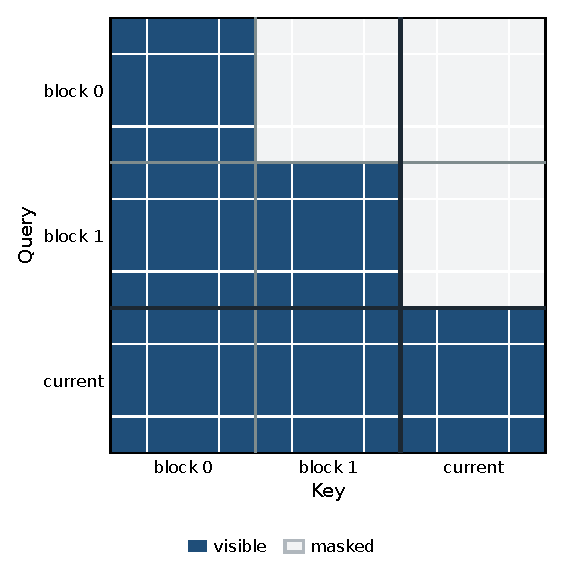
\includegraphics[width=0.48\textwidth]{belf_attn.pdf}
\caption{BELF 一次前向的注意力。查询看行、键看列。}
\label{fig:belf-attn}
\end{figure}

\begin{figure}[H]
\centering
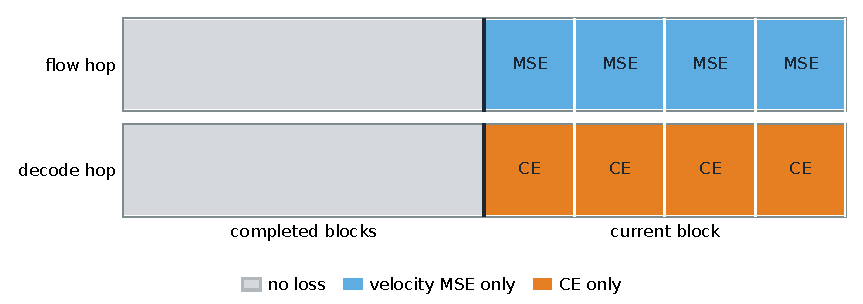
\includegraphics[width=0.72\textwidth]{belf_pack.pdf}
\caption{BELF：已完成的前块不算损失。\(T\) 次流的未知槽都算速度 MSE。橙为末流档（该步 Euler 后读出），仍是 v-MSE。}
\label{fig:belf-pack}
\end{figure}

\paragraph{self-cond 通道。}
未知槽共享同一套 sc。新块起始训练为 0；推理使用上一跳 \(\hat x_0\)。左段与已知槽恒为 0。\(p_{\mathrm{drop}}^{\mathrm{ctx}}\) 只改变注意力。已知槽 AdaLN 仅以 \(t=1\) 为条件，不加 \(m\)、不以 \(w_{\mathrm{sc}}\) 为条件。未知槽以 \(w_{\mathrm{sc}}\) 为条件。

\subsection{推理}

\texttt{block\_generate}。前缀如何切成「完整块进 KV + 当前块左侧已知余数」、每跳如何覆写已知槽、读出后如何提交，见第~\ref{sec:belf-clean}~节。未知槽共 \(T\) 次 \(G\)：跳 \(i=0,\ldots,T-1\) 未知槽 \(t=L_i\)，Euler \(\Delta t=L_{i+1}-L_i\)（末流从 \(L_{T-1}\) 到 \(1-\varepsilon\)）；然后用末次 \(\hat x_0\) 走 VAE-dec。只要仍需续写且总长未到 \texttt{max\_seq\_len}，后续块整块未知（末块可短）。可因 EOS 提前停止。\texttt{sc\_cfg} 为真时：未知槽 sc 使用上一步 \(\hat x_0\)，AdaLN 以推理 \(w_{\mathrm{sc}}\) 为条件；新块起始与已知槽为 \(0\)。采样器见第~\ref{sec:infer}~节。

\subsection{BELF 参数}

{\small
\begin{center}
\begin{tabularx}{\textwidth}{@{}l c X l@{}}
\toprule
名称 & 符号 & 释义 & 默认 \\
\midrule
\multicolumn{4}{@{}l}{\textit{模型}} \\
\texttt{block\_size} & \(W\) & \(G\) 去噪块长。默认见表（100m 为 16）；入口块长独立，须 \(\in\{1,W\}\)；可训档另要求入口块长为 \(1\)。 & \(16\) \\
\texttt{time\_step} & \(T\) & 每块跳数。须 \(T\ge 4\)，否则报错。主跑 \(W=T\)。 & \(16\) \\
\midrule
\multicolumn{4}{@{}l}{\textit{训练}} \\
\texttt{train\_t\_schedule} & & 训练期时间采样规则。 & \texttt{block} \\
\texttt{cond\_mode} & & 当前块内已知余数如何条件化。 & \texttt{clean} \\
\texttt{clean\_block\_prob} & \(p_{\mathrm{clean}}\) & 训练时当前块抽成混合块的概率。不进消融。 & \(0.05\) \\
训练长度 & & \texttt{forward} 要求序列长度被 \(W\) 整除，否则报错。切分档须满足此约束。 & 须整除 \\
\bottomrule
\end{tabularx}
\end{center}
}

所有跳对未知有效位叠加 v-MSE（一律 \(m=\mathrm{denoise}\)，可 CFG）；不引入 \(m_d\)/\(m_c\)。注意力见第~\ref{sec:belf-mask}~节。未知槽同一标量 \(t\)；已知槽钉 \(t=1\)。生成使用 \texttt{block\_generate}。加载入口块长须 \(\in\{1,W\}\)。训练序列长度须被 \(W\) 整除。默认 \(W\) 见表（100m 为 16），主跑 \(W=T\)。\texttt{clean\_block\_prob} 不进消融。全局提交、采样器与温度见第~\ref{sec:infer}~节；CFG 尺度见第~\ref{sec:cfg}~节。

\subsection{BELF 消融}

对照按下列网格执行。全局推理消融见第~\ref{sec:infer}~节。未知槽同一 \(t\)、已知槽钉 \(t=1\)、所有跳未知槽均算 v-MSE 为方法规则，不列入本表。\texttt{clean\_block\_prob} 不进消融。蒸馏方式待定，见第~\ref{sec:open}~节。

{\small
\setlength{\tabcolsep}{4pt}
\begin{center}
\begin{tabularx}{\textwidth}{@{}
  >{\raggedright\arraybackslash}p{0.22\textwidth}
  c
  >{\raggedright\arraybackslash}p{0.16\textwidth}
  >{\raggedright\arraybackslash}X
  @{}}
\toprule
名称 & 符号 & 默认 & 对照 \\
\midrule
\multicolumn{4}{@{}l}{\textit{模型}} \\
\texttt{block\_size} & \(W\) & \(16\) & \(1\)（去噪块长对照） \\
\texttt{time\_step} & \(T\) & \(16\) & \(\{4,8,32\}\)（固定 \(W\)；从零训） \\
\midrule
\multicolumn{4}{@{}l}{\textit{训练}} \\
\texttt{distill\_time\_step} & \(T'\) & （关） & \(\{8,4\}\)（教师 \texttt{time\_step=16}；学生少步；\(W\) 不变。蒸馏方式待定） \\
\bottomrule
\end{tabularx}
\end{center}
}

蒸馏与从零训练少步须分开报告。蒸馏方式待定，见第~\ref{sec:open}~节。主跑不蒸馏。\texttt{block\_size} 去噪块长对照 \(W=1\)；不再扫 \(\{4,8,32\}\)。\texttt{clean\_block\_prob} 不进消融。

\section{RELF}
\label{sec:relf}

滚动半自回归。窗内位置 \(k\) 具有局部时间 \(t_k\)：
\[
z^k=t_k z_0^k+(1-t_k)\varepsilon^k.
\]
主跑下每档 \(S\) 个槽共享同一 \(L_i\)，而非逐槽独立采样时间。加载入口块长必须为 \(1\)（逐 token 因果）。RELF 不声明 \texttt{block\_size}。窗长为 \texttt{window\_size}（\(W\)），与入口块长无关。须 \(T\ge 4\) 且 \(S\cdot T=W\)，否则启动报错拒绝。当前窗已知余数如何自生成、如何训，见第~\ref{sec:relf-clean}~节。

生成分为三段。Freeroll 为滚动阶段：整窗铺 \(F\)，梯子有 \(T\) 档，每档 \(S\) 个槽，最左档 \(t=L_{T-1}\)、右侧纯噪。每步一次 \(G\)：未知档（含最左）各升\textbf{一档}（最左 Euler 到 \(1-\varepsilon\)），用最左该步 \(\hat x_0\) 读出并 pop 这 \(S\) 槽，右端补入 \(S\) 个新噪声，回到 freeroll。\(S\) 只表示档宽与 pop 个数。Preroll / postroll 把同一把 \(F\) 铺在虚拟满窗上：\textbf{BOS 之前整段截掉}、\textbf{EOS 之后整段截掉}；两切可叠加。截断位置由 BOS / EOS 所在格决定。总长上限为 \texttt{max\_seq\_len}。

\subsection{Clean}
\label{sec:relf-clean}

主跑 \texttt{cond\_mode=clean}。本节写窗内已知余数如何自生成、如何训。窗的 \(t\) 场（BOS 前 / EOS 后截 \(F\)）见第~\ref{sec:relf-t}~节；损失见第~\ref{sec:relf-mask}~节。

\paragraph{格子。}
从文档起点按 \(S\) 对齐。前缀长 \(L\)（含 BOS）时 \(r=L\bmod S\)，\(g=\lfloor L/S\rfloor\cdot S\)。完整 pop \([0,g)\) 进入 KV。\(S=1\) 时 \(r\) 恒为 0，不触发余数爬梯。不从任意 \(L\) 另开窗离开 \(S\) 格。

\paragraph{自生成。}
\texttt{rolling\_generate}。新词一律从 \(L_0\) 爬到 \(L_{T-1}\) 再 Euler 到 \(1-\varepsilon\) 才读出 / pop；余数只钉干净，不让新词跳过梯子。
\begin{itemize}
  \item \(L=0\)：preroll。虚拟窗 \(u<i_{\mathrm{bos}}\)，BOS 落在窗内、\textbf{其左截掉}；\(u\) 每次右移 \(S\)，直到 BOS 落到 \(k=0\) 再读出并进入 freeroll。clean 不介入。见图~\ref{fig:relf-emit}。
  \item \(L>0\) 且 \(r=0\) \textbf{且已有} \(z_{\mathrm{carry}}\)：跳过 preroll 与爬梯。当前窗整窗未知，\(t\leftarrow F\)，进入 freeroll。
  \item \(L>0\) 且（\(r>0\) \textbf{或尚无} \(z_{\mathrm{carry}}\)）：\textbf{余数爬梯}（与 preroll 同构）。对齐前缀冷启动 \(r=0\) 时 known 为空、\(n_{\mathrm{write}}=S\)。余数是文档 \([g,g+r)\)。共 \(T\) 帧，hop \(h=0,\ldots,T-1\)：
  \begin{itemize}
    \item 虚拟下标：余数起点 \(k_0=W-S(h+1)=S(T-h-1)\)。窗原点 \(u=g-k_0\)。\(k<k_0\) 的格丢掉（不在当前窗；已写完整 pop 在 KV）。
    \item 槽 \([k_0,k_0+r)\) 为已知（encoder 干净码，\(t=1\)，不进损失）。其余真槽未知，铺各格 \(F_k\)（\(F\) 不滑）。句尾切：EOS 之后仍丢掉。
    \item 每帧一次 \(G\)。\(h<T-1\)：最左流档仍在 \(k_0\) 左侧，已截掉；未知档 Euler 升一档，右端补 \(S\) 个 \(L_0\) 新噪声；\textbf{不 pop}；已知槽覆写 \(t=1\)。
    \item \(h=T-1\)：\(k_0=0\)，即混合满窗 \(F\)。最左档 \(t=L_{T-1}\) 亦 Euler 到 \(1-\varepsilon\)；未知最左格训练算 v-MSE，推理用该步 \(\hat x_0\) 走 VAE-dec 后 pop 这 \(S\) 槽（已知 \(r\) 来自前缀 encoder，新写 \(S-r\) 默认 \(\hat x_0\)）。随后 freeroll，窗内不再带余数。
  \end{itemize}
  \item BOS 若落在已知余数里：钉干净，不当未知，也不踢出窗。
  \item 同一次滚动里刚 pop 的槽走 \texttt{commit\_x0hat}；若下次调用把已写文本当新前缀，完整 pop 先 encode 再提交。
\end{itemize}

\paragraph{训练。}
先取合法窗起点，再按 BOS 前 / EOS 后截 \(F\)（须保住 BOS / EOS，PAD 不当截断对象）。\(r\) 是截断生成：已知为已经写出的真 token；切点必须在 EOS / PAD 之前，且至少留一个未知真槽；\(r\) 不得 \(\ge S\)。
\begin{itemize}
  \item \textbf{不做句首切}：以概率 \texttt{clean\_block\_prob} 抽\textbf{余数爬梯的一帧}（不是只抽末帧）。先抽 \(h\sim\mathrm{Unif}\{0,\ldots,T-1\}\)，再铺该 hop 的左切：\(k_0=S(T-h-1)\)。句首切判定为 \(\mathrm{bos\_cut}=(u+k_0)<i_{\mathrm{bos}}\)（留下的第一格是否仍在 BOS 前），不是 \(u<i_{\mathrm{bos}}\)。记该帧切完后真窗长 \(N'\)（从 \(k_0\) 起到 EOS / 右端）。令 \(r_{\mathrm{hi}}=\min(S-1,N'-1)\)。若 \(r_{\mathrm{hi}}\ge 1\)，则 \(r\sim\mathrm{Unif}\{1,\ldots,r_{\mathrm{hi}}\}\)；已知 \([k_0,k_0+r)\)（encoder 干净码、\(t=1\)），其余真槽未知（各格 \(F_k\)，\(F\) 不滑）。\(h=T-1\) 时 \(k_0=0\)，即混合满窗 \(F\)。\(h<T-1\) 时最左流档已切掉，只监督更噪档 MSE。句尾切：EOS 不当已知。\(N'=1\) 或 \(S=1\) 则不抽。
  \item \textbf{做了句首切}（留下的格仍有 \(j<i_{\mathrm{bos}}\)）：不抽 \(r\)（那是 preroll，BOS 自己爬梯）。不把切掉的左侧改铺 \(t=0\)，也不在更噪的真窗左端再钉干净。两端都切（含句首切）同此。
\end{itemize}
不为凑档截掉 BOS / EOS 或把 PAD 当截断对象。已知槽与左段训练时默认都是 encoder 码（教师强制）；以概率 \texttt{self\_left\_prob} 把左段换成末流 \(\mathrm{sg}(\hat x_0)\)。推理左段默认是自生成的 \(\hat x_0\)。

\paragraph{排除项。}
任意位置填空（左右都有干净上下文）不在本文档范围。禁止把余数钉在满窗 \(F\) 左侧、一次 \(G\) 就读出（新词须走完 \(L_0\to L_{T-1}\) 再 Euler 到 \(1-\varepsilon\)）。

\begin{figure}[H]
\centering
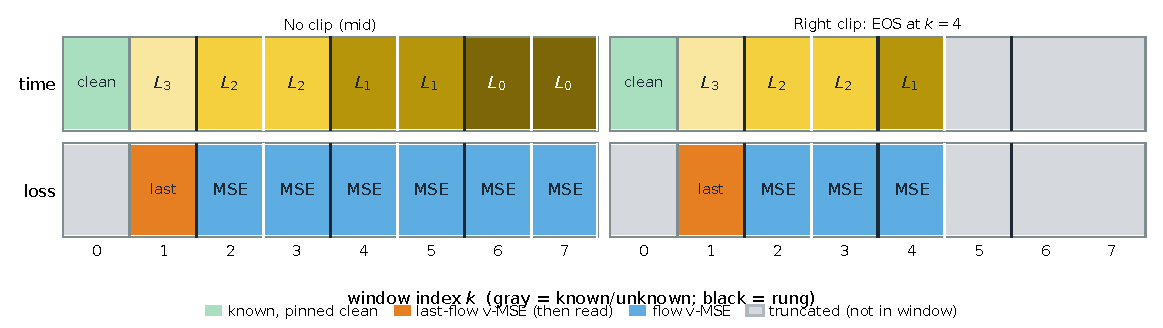
\includegraphics[width=\textwidth]{relf_clean.pdf}
\caption{RELF clean \textbf{末帧}（\(h=T-1\)）：余数已在虚拟 \(k=0\)，最左流档 Euler 后才读出。左列句中满窗；右列句尾切（EOS 后截掉，\(F\) 不滑）。这是爬梯的最后一帧，不是续写全过程。}
\label{fig:relf-clean}
\end{figure}

续写全过程见图~\ref{fig:relf-clean-cont}：这 \(T\) 帧就是 \(L>0,r>0\) 的推理。余数 \(K\) 从虚拟窗右端进入、随 hop 左移 \(S\)；其右第一个新词沿 \(F\) 从 \(L_0\) 升到 \(L_{T-1}\) 再 Euler 到 \(1-\varepsilon\)，全程打 v-MSE，末档才读出 / pop。不画随后的 freeroll。

\begin{figure}[H]
\centering
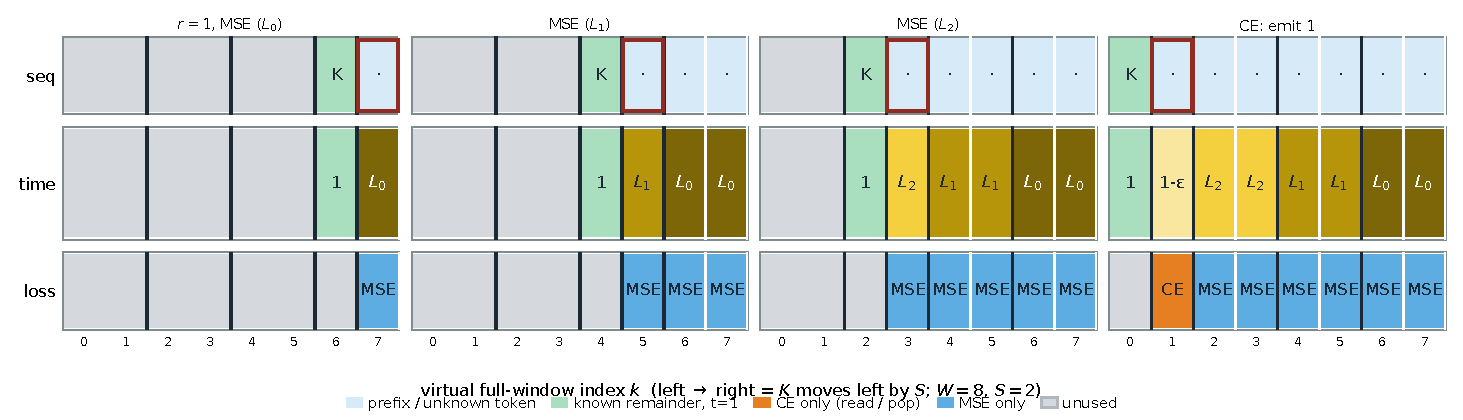
\includegraphics[width=\textwidth]{relf_clean_cont.pdf}
\caption{RELF clean 续写（\(W=8\)，\(S=2\)，\(r=1\)）。虚拟满窗左切：绿格 K 第一帧在 \(k{=}6\)（靠右），之后每次左移 \(S\)。红框为即将读出的新词：全程打 v-MSE，末流档 \(L_{T-1}\) Euler 后才读出。末帧 K 在 \(k{=}0\)，即混合窗 \(F\)，对应图~\ref{fig:relf-clean}。不画第一次 pop 之后的 freeroll。}
\label{fig:relf-clean-cont}
\end{figure}

\subsection{训练}

加载并按 \texttt{latent\_tune} 编码，映射后 2L pack。CFG 采样见第~\ref{sec:cfg}~节（guided 时最右 \(S\) 槽 sc 仍为 \(0\)）。启动时若加载入口块长 \(\neq 1\)，或 \(T<4\)，或 \(S\cdot T\neq W\)，则报错拒绝。按第~\ref{sec:relf-t}~节指定窗内时间：先取合法窗起点，再按 BOS 前 / EOS 后截 \(F\)。是否抽余数爬梯的一帧（未做句首切），见第~\ref{sec:relf-clean}~节。

各槽按所赋 \(t_k\) 独立加噪；已知槽不加噪。损失与注意力按第~\ref{sec:relf-mask}~节排布。未知真槽一律 v-MSE。

接口：\texttt{forward(tokens)} 按当前窗相对序列起止截断铺 \(t\) 场，再计算混合损失。配置为 \texttt{train\_t\_schedule=mixed}。生成使用 \texttt{rolling\_generate}。混合窗见第~\ref{sec:relf-clean}~节。

\subsection{掩码排布}
\label{sec:relf-mask}

一次前向的 pack 是 \(\bigl[\text{左段前缀}\mid\text{右段当前窗}\bigr]\)。窗长 \(W\)，从 0 对齐。一批窗时右段按窗拼接，各窗独立套用下列规则，禁止跨窗右段相互可见。pad 位不进损失，留在 pack 里。左段与已知槽不进入 \(\mathcal{L}\)。须 \(S\cdot T=W\)。

\paragraph{注意力。}
见图~\ref{fig:relf-attn}。与 BELF 同形的是「组内双向、组间单向」：已完成前段的组是加载入口块长（必须为 1，即逐 token 因果）；当前窗的组是档 \(S\)（同一档双向，右档可见左档，左档不可见右档）。窗可见文档位置早于本窗起点的已完成前段；前段不能看窗。一批右段时各窗独立，禁止跨窗互看。\(p_{\mathrm{drop}}^{\mathrm{ctx}}\) 时切断左段。

\begin{figure}[H]
\centering
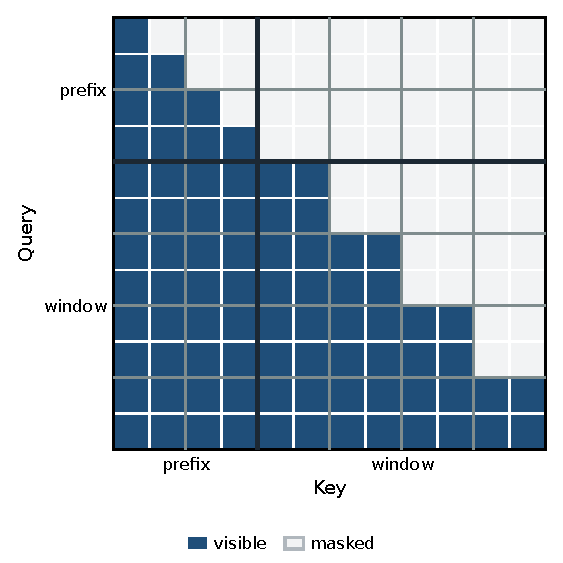
\includegraphics[width=0.48\textwidth]{relf_attn.pdf}
\caption{RELF 一次前向的注意力。查询看行、键看列。}
\label{fig:relf-attn}
\end{figure}

\paragraph{损失。}
仅施加于右段。先按第~\ref{sec:relf-t}~节把 \(F\) 切完，再对\textbf{仍在窗的未知真槽}算 v-MSE。不是按句中 / 句首 / 句尾查表；两种切法叠在同一窗上仍用同一式。已知槽、PAD、以及 BOS 前 / EOS 后丢掉的格不进 \(\mathcal{L}\)。未知真槽一律 \(m=\mathrm{denoise}\)（可 CFG）：
\[
\mathcal{L}
=\lambda_{\mathrm{mse}}\,\frac{\sum_{k\in\mathcal{U}}\|\hat v_k-v_{\mathrm{tgt},k}\|^2}{|\mathcal{U}|},
\]
其中 \(\mathcal{U}\) 为切完后的未知真槽。\(|\mathcal{U}|=0\) 时该项为 0。余数爬梯：\(h<T-1\) 时最左流档在 \(k_0\) 左侧、已切掉，只更噪档 MSE；末帧 \(k_0=0\) 时已知槽仍为 0，最左未知格也算 v-MSE。丢掉的格不加 \(m\)。

\begin{figure}[H]
\centering
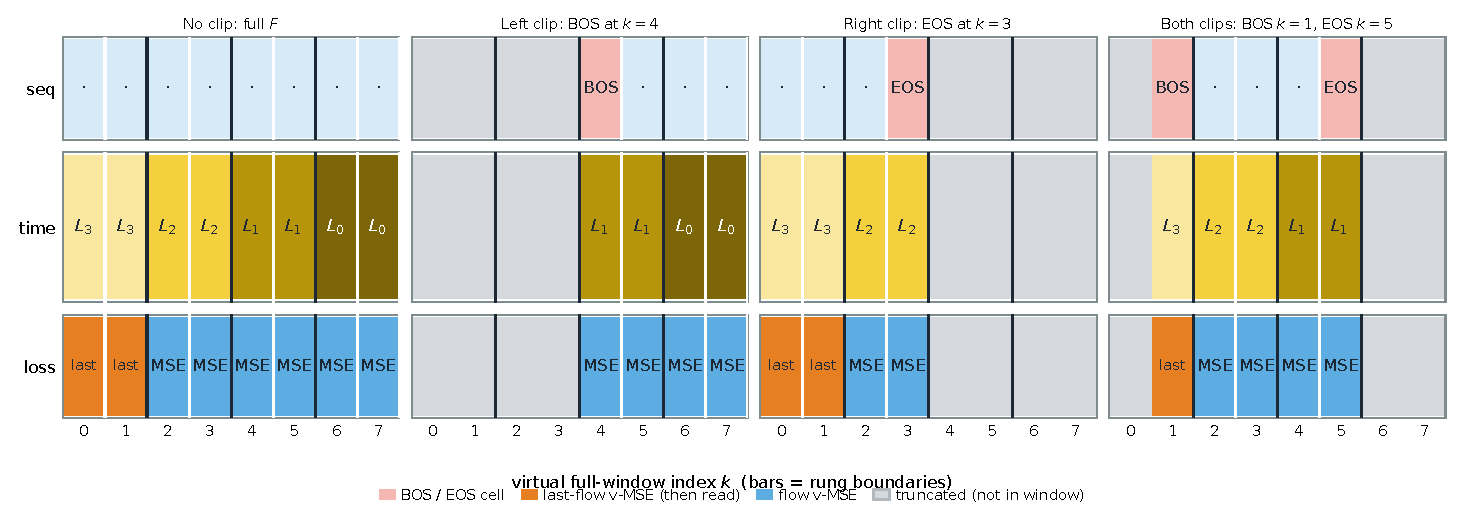
\includegraphics[width=\textwidth]{relf_masks.pdf}
\caption{RELF 画的是虚拟满窗 \(F\)（\(W=8\)，每档 2 槽）。黄净、黑噪。橙=最左流档 \(t=L_{T-1}\)（该步 Euler 到 \(1-\varepsilon\) 后读出）；蓝=更噪流档。灰格是 BOS 之前或 EOS 之后，不在窗、不赋 \(t=0\)。前三列是只切一侧或都不切；右列两端都切。损失按切完后的 \(F_k\) 按格计算，不是三选一。}
\label{fig:relf-masks}
\end{figure}

\paragraph{self-cond 通道。}
右段已有上一跳估计的未知槽写 \(\mathrm{sg}(\hat x_0^{u})\)（guided 时）。最右新进的 \(S\) 个噪声槽 sc 恒为 0。最左档与其余未知档同样以 \(w_{\mathrm{sc}}\) 为条件。左段 / 已知槽 / 干净槽为 0。\(p_{\mathrm{drop}}^{\mathrm{ctx}}\) 只改注意力。已知槽 AdaLN 仅以 \(t=1\) 为条件，不加 \(m\)、不以 \(w_{\mathrm{sc}}\) 为条件。

\subsection{推理}

\texttt{rolling\_generate}。前缀如何切成「完整 pop 进 KV + 余数爬梯」、\(L=0\) 是否 preroll、\(r>0\) 时 \(T\) 帧后才第一次 pop，见第~\ref{sec:relf-clean}~节。接近 \texttt{max\_seq\_len} 或更短目标时改 postroll：EOS 落在窗内，\textbf{其右全部截掉}。PAD 不计、不当边界。EOS 只出现在句尾真槽里。
首词与末词如何落到最左流档再被读出，见图~\ref{fig:relf-emit}。

\begin{figure}[H]
\centering
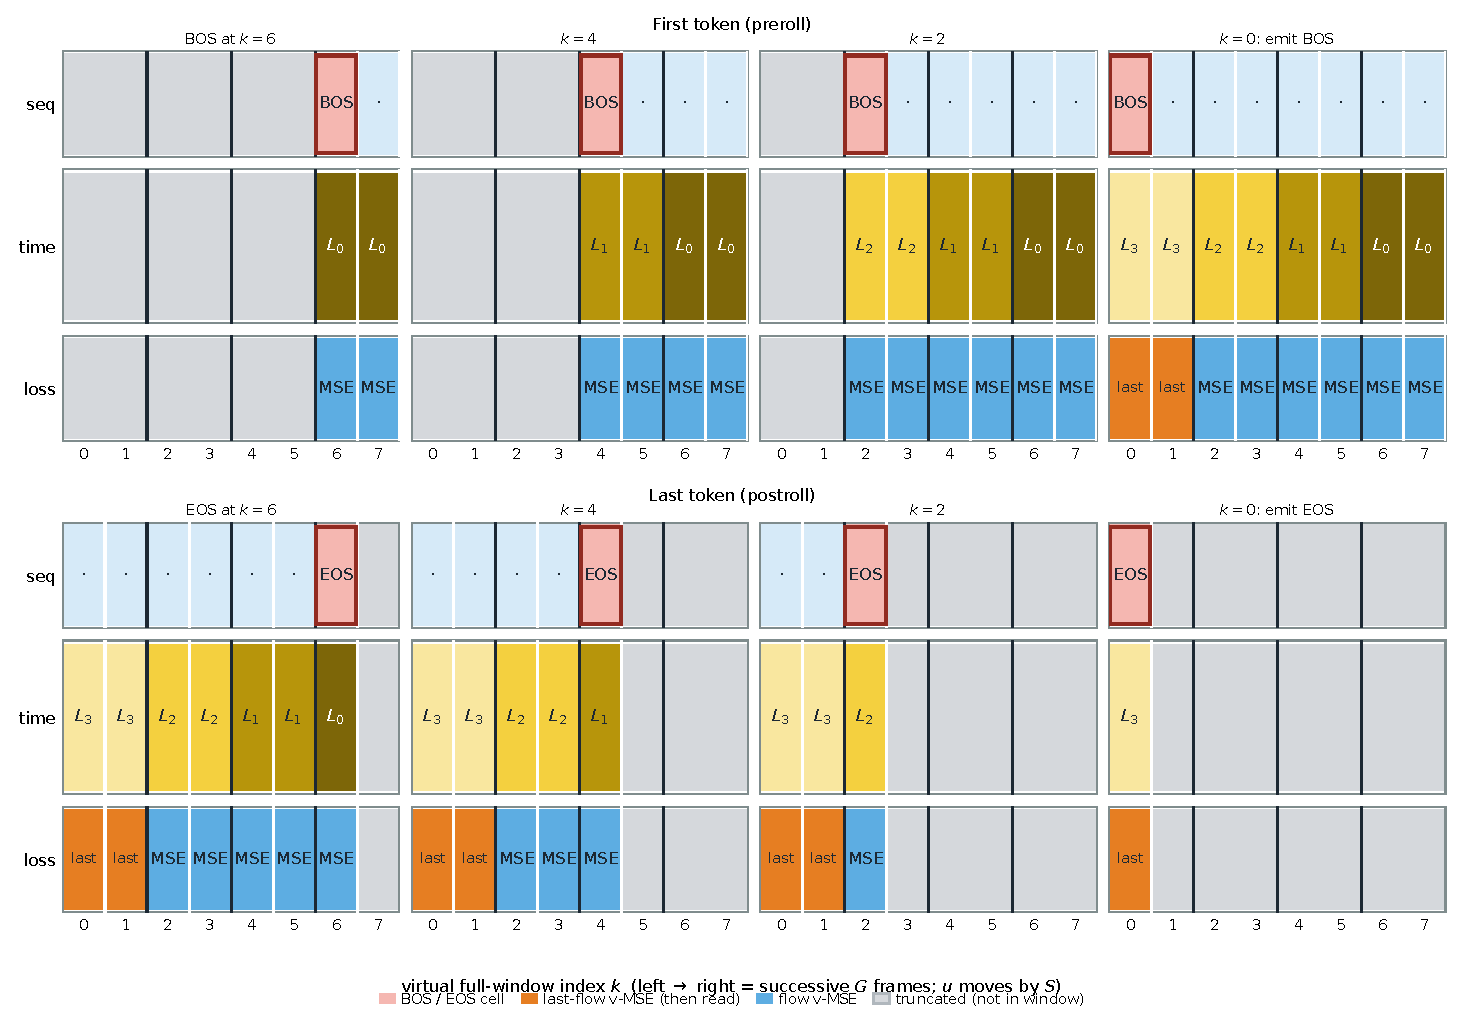
\includegraphics[width=\textwidth]{relf_emit.pdf}
\caption{RELF 推理吐词（\(W=8\)，每档 \(S=2\)）。上行句首切：窗起点 \(u\) 每次右移 \(S\)，BOS 在虚拟满窗上左移；前三帧最左流档仍在 BOS 之前（已截掉），无读出；末帧 BOS 落到 \(k=0\)，该档 Euler 后 VAE-dec 并 pop 出首词。下行句尾切：EOS 之后丢掉、不再右补噪声；EOS 左移，末帧只剩 \(k=0\) 的 EOS，VAE-dec 读出。灰格不在窗，不赋 \(t=0\)。}
\label{fig:relf-emit}
\end{figure}

\texttt{sc\_cfg} 为真时：未知槽 sc 使用上一步提交的 \(\hat x_0\)，AdaLN 以推理 \(w_{\mathrm{sc}}\) 为条件；开局、新进噪声槽与已知槽为 \(0\)。采样器见第~\ref{sec:infer}~节。

\subsection{RELF 参数}

{\small
\begin{center}
\begin{tabularx}{\textwidth}{@{}l c X l@{}}
\toprule
名称 & 符号 & 释义 & 默认 \\
\midrule
\multicolumn{4}{@{}l}{\textit{模型}} \\
\texttt{window\_size} & \(W\) & 滚动窗长。须 \(S\cdot T=W\)。 & \(32\) \\
\texttt{time\_step} & \(T\) & 梯子档数。须 \(T\ge 4\)，否则报错。须 \(S\cdot T=W\)。 & \(16\) \\
\texttt{step\_size} & \(S\) & 每步从窗左端 pop 的槽数，亦为档宽。须 \(S\cdot T=W\)。 & \(2\) \\
\texttt{window\_t} & \(t_k\) & 窗内时间场。锁死 \texttt{ladder}，不进消融。 & \texttt{ladder} \\
\midrule
\multicolumn{4}{@{}l}{\textit{训练}} \\
\texttt{train\_t\_schedule} & & 训练期时间采样规则。 & \texttt{mixed} \\
\texttt{cond\_mode} & & 当前窗内已知余数如何条件化。 & \texttt{clean} \\
\texttt{clean\_block\_prob} & \(p_{\mathrm{clean}}\) & 未做句首切时抽余数爬梯一帧的概率（含 hop \(h\) 与 \(r\)；切点在 EOS 前）。不进消融。 & \(0.05\) \\
\bottomrule
\end{tabularx}
\end{center}
}

生成使用 \texttt{rolling\_generate}。窗的 \(t\) 场由句首切 / 句尾切对整窗 \(F\) 给出，两切可叠加，不另设分支概率。余数爬梯见第~\ref{sec:relf-clean}~节。未知真槽一律 v-MSE（窗内最高档为 \(t=L_{T-1}\)，不是 \(1-\varepsilon\)），不进参数、不进消融。\texttt{window\_t} 锁死 \texttt{ladder}，不进消融。\texttt{clean\_block\_prob} 不进消融。消融见下表。全局提交、采样器与温度见第~\ref{sec:infer}~节；CFG 尺度见第~\ref{sec:cfg}~节。

\subsection{RELF 消融}

对照按下列网格执行。改 \(W\) 时须保持 \(T\ge 4\) 且 \(S\cdot T=W\)。全局推理消融见第~\ref{sec:infer}~节。未知真槽一律 v-MSE，不进消融。\texttt{window\_t} 锁死 \texttt{ladder}，不进消融。\texttt{clean\_block\_prob} 不进消融。蒸馏方式待定，见第~\ref{sec:open}~节。

{\small
\setlength{\tabcolsep}{4pt}
\begin{center}
\begin{tabularx}{\textwidth}{@{}
  >{\raggedright\arraybackslash}p{0.22\textwidth}
  c
  >{\raggedright\arraybackslash}p{0.16\textwidth}
  >{\raggedright\arraybackslash}X
  @{}}
\toprule
名称 & 符号 & 默认 & 对照 \\
\midrule
\multicolumn{4}{@{}l}{\textit{模型}} \\
\texttt{window\_size} & \(W\) & \(32\) & 改 \(W\) 时同步改 \(T\) 或 \(S\)（须 \(S\cdot T=W\)） \\
\texttt{step\_size} & \(S\) & \(2\) & \(1\)（须 \(T=W/S\)） \\
\midrule
\multicolumn{4}{@{}l}{\textit{训练}} \\
\texttt{distill\_time\_step} & \(T'\) & （关） & \(\{8,4\}\)（教师 \texttt{time\_step=16}；学生少步；\texttt{window\_size} 不变，须 \(S\cdot T'=W\)。蒸馏方式待定） \\
\bottomrule
\end{tabularx}
\end{center}
}

蒸馏与从零训练少步须分开报告。蒸馏方式待定，见第~\ref{sec:open}~节。主跑不蒸馏。改 \(T'\) 时 \texttt{window\_size} 不变，则同步改 \texttt{step\_size} 以保持 \(S\cdot T'=W\)。

\section{推理}
\label{sec:infer}

本节给出两族共用的推理项。这些字段可在同一 checkpoint 上更改，不进入训练指纹。BELF 生成使用 \texttt{block\_generate}，RELF 生成使用 \texttt{rolling\_generate}。CFG 的推理尺度见第~\ref{sec:cfg}~节。

默认 \texttt{commit\_x0hat=false}：先由 VAE-dec 读出 token，再 encode \textbf{采 \(z\)}（\texttt{sample=(x0\_source==z)}）写入，空间与 \texttt{x0\_source} 一致。对照 \texttt{true}：将 \(G\) 的 \(\hat x_0\)（流空间 \(X\)）写入 \(G\) 的 KV。外部前缀完整块仍走 encoder、\texttt{sample=false}。两条策略分开报告。训练时左段默认是 encoder 的干净码，以概率 \texttt{self\_left\_prob} 换成末流 \(\mathrm{sg}(\hat x_0)\)。VAE-dec 无状态，不维护 KV。提交时左段 \(t=1\)，AdaLN 不以 \(w_{\mathrm{sc}}\) 为条件，sc 通道为 0。

采样默认 \texttt{sampling\_method=sde}（\(\gamma\) 见表），对照 \texttt{ode}。\texttt{sde} 时 churn 关在最后一次\textbf{流}（BELF 跳 \(T-1\)；RELF 升档侧，含最左末流）。\texttt{sc\_cfg} 为真时，未知槽 AdaLN 以推理 \(w_{\mathrm{sc}}\) 为条件（仅开训 checkpoint 可扫描）。前缀 KV 不随 \(w_{\mathrm{sc}}\) 重算。

\subsection{推理参数（全局）}

{\small
\begin{center}
\begin{tabularx}{\textwidth}{@{}l c X l@{}}
\toprule
名称 & 符号 & 释义 & 默认 \\
\midrule
\multicolumn{4}{@{}l}{\textit{推理}} \\
\texttt{commit\_x0hat} & & 关则再 encode 采 \(z\)；开则提交 \(\hat x_0\)。 & \texttt{false} \\
\texttt{sampling\_method} & & \texttt{sde} 或 \texttt{ode}。 & \texttt{sde} \\
\texttt{sde\_gamma} & \(\gamma\) & 仅 \texttt{sde} 的噪声系数。 & \(1.5\) \\
\texttt{temperature} & & 出口温度；\(\le 0\) 为 argmax。 & \(0.0\) \\
\bottomrule
\end{tabularx}
\end{center}
}

\subsection{推理消融（全局，不重训）}

对照按下列网格执行。同一 checkpoint。\(w_{\mathrm{sc}}\) / \(w_{\mathrm{ctx}}\) 扫描见第~\ref{sec:cfg}~节。评测长度见附录~\ref{sec:len}。\texttt{sde\_gamma} 取值对齐 ELF 已报告的工作点：论文默认 \(1.0\)；32 步设定 \(1.5\)（本文档默认）；8/16 步设定 \(2.0\)。\(\gamma=0\) 时 SDE 退化为 ODE，与 \texttt{sampling\_method=ode} 等价，故消融不另列 \(\gamma=0\)。

{\small
\setlength{\tabcolsep}{4pt}
\begin{center}
\begin{tabularx}{\textwidth}{@{}
  >{\raggedright\arraybackslash}p{0.22\textwidth}
  c
  >{\raggedright\arraybackslash}p{0.16\textwidth}
  >{\raggedright\arraybackslash}X
  @{}}
\toprule
名称 & 符号 & 默认 & 对照 \\
\midrule
\multicolumn{4}{@{}l}{\textit{推理}} \\
\texttt{commit\_x0hat} & & \texttt{false} & 提交 \(\hat x_0\) \\
\texttt{sampling\_method} & & \texttt{sde} & \texttt{ode} \\
\texttt{sde\_gamma} & \(\gamma\) & \(1.5\) & \(\{1.0,1.5,2.0\}\)；仅 \texttt{sde} \\
\bottomrule
\end{tabularx}
\end{center}
}

\section{设计选择与未决项}
\label{sec:open}

前面各章给出已确定的做法。本章记录已闭合的设计选择，以及仍未确定的项。其中「出口 CE」与「左条件暴露偏差」两项以\textbf{问题 / 解决方案}对陈述；其余小节仍为直接结论。

\subsection{已确定：\texorpdfstring{\(w_{\mathrm{sc}}\)}{w\_sc} 进入哪一段 AdaLN}

左段是 \(t=1\) 的干净前缀。若 AdaLN 亦以推理 \(w_{\mathrm{sc}}\) 为条件，前缀 KV 会随 \(w_{\mathrm{sc}}\) 变化，与训练中「左段不以 \(w_{\mathrm{sc}}\) 为条件」不一致。规格如下：\textbf{仅右段未知槽以 \((t,w_{\mathrm{sc}},m=\mathrm{denoise})\) 为条件}。不再设 \(m=\mathrm{decode}\)。提交、左段与已知槽均不以 \(w_{\mathrm{sc}}\) 为条件、不加 \(m\)。\(g=0\) 时 sc 仍为 \(0\)，但未知槽 AdaLN 仍以已采样的 \(w_{\mathrm{sc}}\) 为条件。扫描 \(w_{\mathrm{sc}}\) 时不重算前缀 KV。见第~\ref{sec:cfg}~节、第~\ref{sec:infer}~节。

\subsection{已确定：BELF / RELF 用 clean 处理已知余数}

主跑 \texttt{cond\_mode=clean}。自生成与训练抽样见第~\ref{sec:belf-clean}~节、第~\ref{sec:relf-clean}~节，此处不复述。RELF：未做句首切时抽余数爬梯的一帧（\(h\sim\mathrm{Unif}\{0,\ldots,T-1\}\)，新词从 \(L_0\) 爬到 \(L_{T-1}\) 再 Euler 到 \(1-\varepsilon\) 才读出 / pop）；句首切不抽 \(r\)。禁止钉满窗 \(F\) 左侧一次读出。任意位置填空不在本文档范围。已确定。

\subsection{已确定：出口 CE / decode hop 拉坏流训练}

\textbf{问题。}
旧规格在 \(T-1\) 次流之外另留一档 decode hop：在 \(t=1-\varepsilon\) 再跑 \(G\)，并对出口打 token CE（\texttt{lambda\_ce} / \texttt{ce\_detach\_g} / \texttt{exit}）。CE 与 v-MSE 目标不一致，容易把流场与读出拉向不同方向；评测若用出口 CE 充当 PPL，还会与推理真正走的 TriFluency / Gen.PPL 脱节。梯子按 \(Q(i/(T-1))\) 均分时，分母与「多一档 CE」绑在一起，去掉 CE 后若不改梯子会少一档流。

\textbf{解决方案。}
主体 \(\mathcal{L}\) 只保留 v-MSE（无 \texttt{lambda\_ce} / \texttt{ce\_detach\_g} / \texttt{exit} / \texttt{linear}）。出口锁死为 \(\hat x_0\in X\) 再走加载的 VAE-dec：训练主体不算 CE；VAE-dec 只在推理读出与可训档 \(\mathcal{L}_{\mathrm{s1}}\) 重建里出现。\(G\) 仍一份（禁止 ELF \texttt{decoder\_prob} 双模式）。梯子与 hop 对齐：
\begin{itemize}
  \item \(T\) 是流步数：\(L_i=Q(i/T)\)，\(i=0,\ldots,T\)（\(T+1\) 个点）。不再另留一档 CE / decode hop。
  \item BELF：跳 \(i=0,\ldots,T-1\) 未知槽一律 v-MSE（可 CFG）；推理 \(T\) 次 Euler 后用末次 \(\hat x_0\) 走 VAE-dec。
  \item RELF：仍在窗的未知真槽一律 v-MSE（可 CFG）。最左档 \(t=L_{T-1}\)，该步 Euler 到 \(1-\varepsilon\) 后读出 / pop。两种切法可叠加，损失按格、不按三行表。
  \item AdaLN-Zero 逐列 \((t,w_{\mathrm{sc}},m=\mathrm{denoise})\)。\(m\) 仅未知真槽；不再设 \(m=\mathrm{decode}\)。BOS 前 / EOS 后不在窗，与满窗右侧 \(L_0=0\) 的 denoise 真槽不是一回事。
  \item 主指标沿用仓库 TriFluency / Gen.PPL，不再用出口 CE 充当 eval PPL。
\end{itemize}
训练插值 \(z\) 与推理 Euler \(z\) 的轨迹缺口仍在；左条件暴露偏差见下一对。已确定。

\subsection{已确定：左条件暴露偏差（self-left）}

\textbf{问题。}
链式法则写的是 \(p_G(z^{(b)}\mid z^{(<b)})\)。推理左段默认是再 encode 采 \(z\)（对照 \texttt{commit\_x0hat}）；训练若始终喂 encoder 干净码（教师强制），则右段去噪习惯「完美前缀」，一到推理左边带自生成误差就崩。这是左条件上的暴露偏差。用当前训练 hop（随机 \(t\)）的 \(\hat x_0\) 冒充左段也不行：离提交码太远。块内已知余数与 PAD 另有钉干净规则，不应拿 \(\hat x_0\) 冒充。

\textbf{解决方案。}
以概率 \texttt{self\_left\_prob}（默认 \(0.25\)，eval / 生成视为 0）做 self-left scheduled sampling：在 CFG 之前，用 GT 左 + 右段钉 \(t=L_{T-1}\)、\(m=\mathrm{denoise}\) 做一次 \texttt{no\_grad} \(G\)（与推理末跳同条件，取 x-pred，不 Euler），按样本 Bernoulli 把 \(h_{\mathrm{left}}\) 换成 \textbf{stop-grad 的末流 \(\hat x_0\)}，再跑 teacher / 学生。已知余数与 PAD 仍钉 encoder 干净码。BELF 与 RELF 共用。消融 \(\{0,0.125,0.25,0.375,0.5\}\)。它不消除「插值 \(z\) vs Euler \(z\)」那条缺口，只缓解左条件分布差。机制见第~\ref{sec:self-left}~节。已确定。

\subsection{已确定：日程档 \texttt{mid}}

checkpoint 变体 \texttt{fast} / \texttt{mid} / \texttt{full} 与 \texttt{latent\_tune=mid}（15B 解冻）不是同一键。日程档 \texttt{mid} 仅 Stage1：全局序列批 128、主预算 \(10\mathrm{B}\)、\texttt{eval\_step}=1000、\texttt{ema\_decay}=0.999，用于中档验证，无 Stage2。路径 \texttt{cache/checkpoints/mid/\ldots}。已确定。

\subsection{未决：少步蒸馏}

两族消融都列 \texttt{distill\_time\_step} \(\{8,4\}\)（教师 \(T=16\)），与从零训少步分开报告。主跑不蒸馏。蒸馏配方尚未确定：是否冻结已训教师、学生改哪些参数、损失如何书写，两族同一未决项。RELF 还须保持 \(S\cdot T'=W\)。

\appendix
\section{长度日程}
\label{sec:len}

切分仅用于构造训练样本。模型只声明 \texttt{max\_seq\_len}=4096。

\begin{itemize}
  \item 日程档 \texttt{full} / \texttt{mid} 的 Stage1 对齐长度 512，全部样本为该长度。\texttt{full} 全局批 512；\texttt{mid} 全局批 128、预算 \(10\mathrm{B}\)、\texttt{eval\_step}=1000，无 Stage2。
  \item 日程档 \texttt{full} 的扩展对齐长度 2048；\(5\mathrm{B}\) 按档 token 比 \(1{:}2{:}3{:}4\) 分成 \(0.5{+}1.0{+}1.5{+}2.0\,\mathrm{B}\)，档 \(\{256,512,1024,2048\}\)。
  \item 训练切分止于 2048。\(2048<S\le 4096\) 仅出现于推理外推。eval 主报 2048，4096 作为外推。主指标沿用仓库 TriFluency / Gen.PPL，不再用出口 CE 充当 eval PPL。
  \item BELF 训练另要求每条样本长度被 \(W\) 整除（100m 默认 \(W=16\)；上列档均满足）。不整除则 \texttt{forward} 报错。RELF 无此整除约束。
\end{itemize}

\section{共性参数附表}

下列为共性章未列入主表的字段，仍按模型 / 训练 / 推理分栏。CFG 主表见第~\ref{sec:cfg}~节，全局推理主表见第~\ref{sec:infer}~节。修改这些字段仍须写入对应指纹（推理类除外），但本文档不以它们为对照轴。入口 encoder / decoder 只记 \texttt{latent\_model} 与 \texttt{tag}；隐维、词表、VAE 容量、s1 系数以加载结果为准，不列入本表。出口锁死 VAE-dec，无层数键、无 \texttt{linear}。表中 100m 数字供该规模实现对齐，并非另一套规范。BELF 的 \texttt{block\_size}、RELF 的窗字段在本族章，不在本表。

{\small
\setlength{\tabcolsep}{4pt}
\begin{longtable}{@{}
  >{\raggedright\arraybackslash}p{0.24\textwidth}
  >{\centering\arraybackslash}p{0.10\textwidth}
  >{\raggedright\arraybackslash}p{0.42\textwidth}
  >{\raggedright\arraybackslash}p{0.16\textwidth}@{}}
\toprule
名称 & 符号 & 释义 & 默认 \\
\midrule
\endfirsthead
\toprule
名称 & 符号 & 释义 & 默认 \\
\midrule
\endhead
\bottomrule
\endlastfoot
\multicolumn{4}{@{}l}{\textit{模型}} \\
\texttt{proj\_bias} & & 映射是否带偏置。 & \texttt{true} \\
\texttt{proj\_norm} & & 映射后是否 RMSNorm。 & \texttt{rmsnorm} \\
\texttt{whiten} & & 映射前逐维仿射标准化。 & \texttt{true} \\
\texttt{whiten\_on} & & 白化统计对象。 & \texttt{mu} \\
\texttt{n\_layer} & & AdaLN-Zero Transformer 层数。 & \(12\) \\
\texttt{n\_head} & & 头数。须整除 \texttt{n\_embd}。 & \(12\) \\
\texttt{mlp\_ratio} & & SwiGLU 扩展比。 & \(4.0\) \\
\texttt{dropout} & & 注意力 / FFN dropout。 & \(0.0\) \\
\texttt{qk\_norm} & & Q/K 每头 RMSNorm。 & \texttt{true} \\
\texttt{rope\_theta} & \(\theta\) & RoPE 基频。 & \(10000\) \\
\texttt{t\_freq\_dim} & & 正弦时间嵌入频率维。 & \(256\) \\
\texttt{ada\_ln} & & 主跑 AdaLN-Zero（无仿射 LN、残差 gate、调制末层与 FinalLayer 输出线性零初始化）。逐列 \((t,w_{\mathrm{sc}},m)\)；未知一律 \(m=\mathrm{denoise}\)，\texttt{sc\_cfg} 为真时再以 \(w_{\mathrm{sc}}\) 为条件。不再设 \(m=\mathrm{decode}\)。左段与已知槽 \(t=1\)、不加 \(m\)、不以 \(w_{\mathrm{sc}}\) 为条件。不用 ELF in-context。不进消融。 & \texttt{true} \\
\texttt{num\_time\_tokens} & & 整句时间前缀个数。0=条件只走 AdaLN-Zero。 & \(0\) \\
\texttt{right\_attn} & & 2L 右段内部注意力。 & \texttt{bidirectional} \\
\texttt{self\_cond\_mode} & & self-cond 通道接入方式。 & \texttt{concat}（\(2D\to D\)） \\
\texttt{num\_self\_cond\_cfg\_tokens} & & CFG prefix 个数。本规格为 \(0\)。 & \(0\) \\
\texttt{noise\_sigma} & \(\sigma\) & 加噪标准差。 & \(1.0\) \\
\midrule
\multicolumn{4}{@{}l}{\textit{训练}} \\
\texttt{self\_cond\_cfg\_min} & \(w^{\mathrm{sc}}_{\min}\) & 训练 \(w_{\mathrm{sc}}\) 区间下界。 & \(0.5\) \\
\texttt{self\_cond\_cfg\_max} & \(w^{\mathrm{sc}}_{\max}\) & 训练 \(w_{\mathrm{sc}}\) 区间上界。 & \(5.0\) \\
\texttt{vel\_eps} & \(\varepsilon_t\) & 速度分母 \(\max(1-t,\varepsilon_t)\) 的下界。 & \(10^{-3}\) \\
\texttt{lambda\_mse} & \(\lambda_{\mathrm{mse}}\) & v-MSE 系数。无 \texttt{lambda\_ce}。 & \(1.0\) \\
\texttt{ctx\_source} & & 2L 左段用 \(z\) 还是 \(\mu\)。 & \texttt{z} \\
\texttt{x0\_source} & & 流的干净端 / v-MSE 靶。 & \texttt{z} \\
\texttt{optimizer.dtype} & & 训练精度。与 ELF 配方相同。 & \texttt{bf16} \\
\texttt{learning\_rate} & & AdamW 学习率。与 ELF 配方相同。 & \(0.002\) \\
\texttt{muon\_learning\_rate} & & Muon 学习率。与 ELF 配方相同。 & \(0.002\) \\
\texttt{weight\_decay} & & weight decay。 & \(0\) \\
\texttt{muon\_weight\_decay} & & Muon weight decay。 & \(0\) \\
\texttt{beta1} & \(\beta_1\) & AdamW \(\beta_1\)。 & \(0.9\) \\
\texttt{beta2} & \(\beta_2\) & AdamW \(\beta_2\)。 & \(0.95\) \\
\texttt{grad\_clip} & & 全局梯度裁剪。 & \(1.0\) \\
\texttt{muon\_momentum} & & Muon momentum。 & \(0.95\) \\
\texttt{muon\_ns\_steps} & & Muon Newton–Schulz 步数。 & \(5\) \\
\texttt{use\_muon} & & 隐藏层 Linear 用 Muon。 & \texttt{true} \\
\texttt{ema\_decay} & & EMA；\(0\) 关闭。日程档 \texttt{full}/\texttt{fast} 为 \(0.9999\)；日程档 \texttt{mid} 为 \(0.999\)。 & \(0.9999\)（full） \\
\texttt{warmup\_ratio} & & 预热占 \texttt{max\_steps} 的比例。 & \(0.005\) \\
\texttt{min\_lr\_ratio} & & 最小学习率相对峰值；\(1\)=constant（BELF/RELF 脚本 \texttt{--set}）。 & \(1.0\) \\
\texttt{global\_batch\_size} & & 全局批。日程档 \texttt{full} 的 s1 为 512；s2 用 curriculum \texttt{global\_seq\_batch}=128。日程档 \texttt{mid} 的 s1 为 128。 & \(512\)（full s1） \\
\texttt{eval\_step} & & 评测间隔（优化器步）。日程档 \texttt{full} 为 500；日程档 \texttt{mid} 为 1000（全局批更小）。 & \(500\)（full） \\
\midrule
\multicolumn{4}{@{}l}{\textit{推理}} \\
\texttt{ctx\_cfg\_min} & \(w^{\mathrm{ctx}}_{\min}\) & 推理 \(w_{\mathrm{ctx}}\) 下界。 & \(1\) \\
\texttt{ctx\_cfg\_max} & \(w^{\mathrm{ctx}}_{\max}\) & 推理 \(w_{\mathrm{ctx}}\) 上界。 & \(7\) \\
\end{longtable}
}

{\raggedright\printbibliography}
\end{document}
